%% 
%% Copyright 2007-2020 Elsevier Ltd
%% 
%% This file is part of the 'Elsarticle Bundle'.
%% ---------------------------------------------
%% 
%% It may be distributed under the conditions of the LaTeX Project Public
%% License, either version 1.3 of this license or (at your option) any
%% later version.  The latest version of this license is in
%%    http://www.latex-project.org/lppl.txt
%% and version 1.3 or later is part of all distributions of LaTeX
%% version 1999/12/01 or later.
%% 
%% The list of all files belonging to the 'Elsarticle Bundle' is
%% given in the file `manifest.txt'.
%% 
%% Template article for Elsevier's document class `elsarticle'
%% with harvard style bibliographic references

\documentclass[preprint,12pt]{elsarticle}

%% Use the option review to obtain double line spacing
%% \documentclass[preprint,review,12pt]{elsarticle}

%% Use the options 1p,twocolumn; 3p; 3p,twocolumn; 5p; or 5p,twocolumn
%% for a journal layout:
%% \documentclass[final,1p,times]{elsarticle}
%% \documentclass[final,1p,times,twocolumn]{elsarticle}
%% \documentclass[final,3p,times]{elsarticle}
%% \documentclass[final,3p,times,twocolumn]{elsarticle}
%% \documentclass[final,5p,times]{elsarticle}
%% \documentclass[final,5p,times,twocolumn]{elsarticle}

%% For including figures, graphicx.sty has been loaded in
%% elsarticle.cls. If you prefer to use the old commands
%% please give \usepackage{epsfig}

%% The amssymb package provides various useful mathematical symbols
\usepackage{amssymb}
%% The amsmath package provides various useful equation environments.
\usepackage{amsmath}
\usepackage{graphicx}
\graphicspath{{fig/}}
\usepackage{tikz}
\usepackage{float}
\usepackage{booktabs}
\usepackage{graphicx}
\usepackage{caption}
\usepackage{subcaption}
\usepackage{algorithm}
\usepackage{algpseudocode}
\usepackage{xcolor}
% \usepackage[numbers,sort]{natbib}
\usepackage{hyperref}
\usepackage{placeins}
\usepackage{amssymb}
%% The amsthm package provides extended theorem environments
%% \usepackage{amsthm}
% 让引用变成 作者-年份
\biboptions{authoryear,round}  % round=圆括号; 也可加 sort&compress 等
%% The lineno packages adds line numbers. Start line numbering with
%% \begin{linenumbers}, end it with \end{linenumbers}. Or switch it on
%% for the whole article with \linenumbers.
\usepackage{lineno}
\linenumbers
\setlength{\emergencystretch}{2em}

\newif\ifanonymous
\anonymousfalse

\newcommand{\rev}[1]{\textcolor{blue}{#1}}
\newcommand{\revb}[1]{{\color{blue}{#1}}}
\newcommand{\revfloat}{\color{blue}\captionsetup{font={color=blue},labelfont={color=blue}}}
\newcommand{\hl}[1]{\textcolor{red}{#1}}
\newcommand{\hlb}[1]{\textcolor{red}{[#1]}}

\journal{Computers, Environment and Urban Systems}

\begin{document}

\begin{frontmatter}

%% Title, authors and addresses

%% use the tnoteref command within \title for footnotes;
%% use the tnotetext command for theassociated footnote;
%% use the fnref command within \author or \affiliation for footnotes;
%% use the fntext command for theassociated footnote;
%% use the corref command within \author for corresponding author footnotes;
%% use the cortext command for theassociated footnote;
%% use the ead command for the email address,
%% and the form \ead[url] for the home page:
%% \title{Title\tnoteref{label1}}
%% \tnotetext[label1]{}
%% \author{Name\corref{cor1}\fnref{label2}}
%% \ead{email address}
%% \ead[url]{home page}
%% \fntext[label2]{}
%% \cortext[cor1]{}
%% \affiliation{organization={},
%%             addressline={},
%%             city={},
%%             postcode={},
%%             state={},
%%             country={}}
%% \fntext[label3]{}

\title{A Novel Simulation-based Approach to Optimizing Road Networks for Disaster Evacuation in Dense Urban Informal Settlements} %% Article title

%% use optional labels to link authors explicitly to addresses:
%% \author[label1,label2]{}
%% \affiliation[label1]{organization={},
%%             addressline={},
%%             city={},
%%             postcode={},
%%             state={},
%%             country={}}
%%
%% \affiliation[label2]{organization={},
%%             addressline={},
%%             city={},
%%             postcode={},
%%             state={},
%%             country={}}

% Elsevier template: \documentclass{elsarticle}
% Put this inside \begin{frontmatter} ... \end{frontmatter}

\ifanonymous
% \author{Anonymous Submission}
\else
\author[aff1]{Chun Song}
\author[aff1]{Zhijie Zhou}
\author[aff1]{Rui Cao\corref{cor1}}

\affiliation[aff1]{
  organization={Thrust of Urban Governance and Design, Society Hub, The Hong Kong University of Science and Technology (Guangzhou)},
  city={Guangzhou},
  country={China}
}

\cortext[cor1]{Corresponding author.}
\ead{ruicao@hkust-gz.edu.cn}
\fi

%% Abstract
\begin{abstract}
Urban informal settlements in China are often characterized by dense buildings and populations, narrow alleys, and intricate road networks. These features present significant safety challenges and complicate evacuation planning due to their high vulnerability to disasters and the difficulty of large-scale reconstruction. To address the challenges, we propose a coupled simulation-optimization framework designed to evaluate and enhance the road-network performance in these dense informal settlements, thereby improving their disaster-evacuation resilience. By integrating GIS-based environmental reconstruction, potential-field navigation, and a Smoothed Particle Hydrodynamics (SPH)-based crowd density and movement model, the framework accurately simulates pedestrian dynamics. \revb{The movement model is calibrated and validated against empirical corridor-level fundamental-diagram data, while paired multi-seed village-scale simulations and plausibility checks are used to examine the consistency of the resulting evacuation patterns.} Then, a multi-objective optimization algorithm is further used to identify optimal micro-regeneration strategies that balance evacuation efficiency with reconstruction cost. \revb{Sensitivity analyses of crowd-model and optimization parameters are further conducted to assess the robustness of evacuation performance and intervention selection.} A case study conducted in Shipai Village, a dense informal settlement in Guangzhou, China, demonstrates that this approach effectively pinpoints critical network bottlenecks. The optimized intervention achieves a significant reduction in total evacuation time while requiring only minor structural modifications. These findings offer practical and cost-effective guidance for urban planners seeking to improve the resilience and safety of urban informal settlements.
\end{abstract}

%%Graphical abstract
% \begin{graphicalabstract}
%\includegraphics{fig/grabs.png}



% \end{graphicalabstract}





%% Keywords
\begin{keyword}
% Urban Village \ Micro-regeneration  \ Multi-objective Optimization \ Crowd Simulation \ Sustainable Development Goals (SDG) \ Disaster Response \ Urban Resilience
Informal Settlements; Disaster Response; Urban Regeneration; Multi-objective Optimization; Crowd Simulation; Sustainable Development Goals (SDG)
\end{keyword}

\end{frontmatter}

%% Add \usepackage{lineno} before \begin{document} and uncomment 
%% following line to enable line numbers
%% \linenumbers

%% main text
%%

% \textbf{Highlight}
% \begin{itemize}
%     \item Proposing a coupled simulation–optimization framework for micro-regeneration in dense informal settlements.
%     \item Building a high-resolution GIS-to-raster environment and global navigation field for large-scale evacuation simulation.
%     \item Using time and congestion metrics with a weighted objective to balance efficiency and renovation cost.
%     \item Applying a genetic algorithm to search feasible alley interventions and identify key bottlenecks.
%     \item Validating on Shipai Village (Guangzhou) with significant evacuation gains from minor upgrades.
% \end{itemize}




\section{Introduction}
\begin{figure}[t]
    \centering
    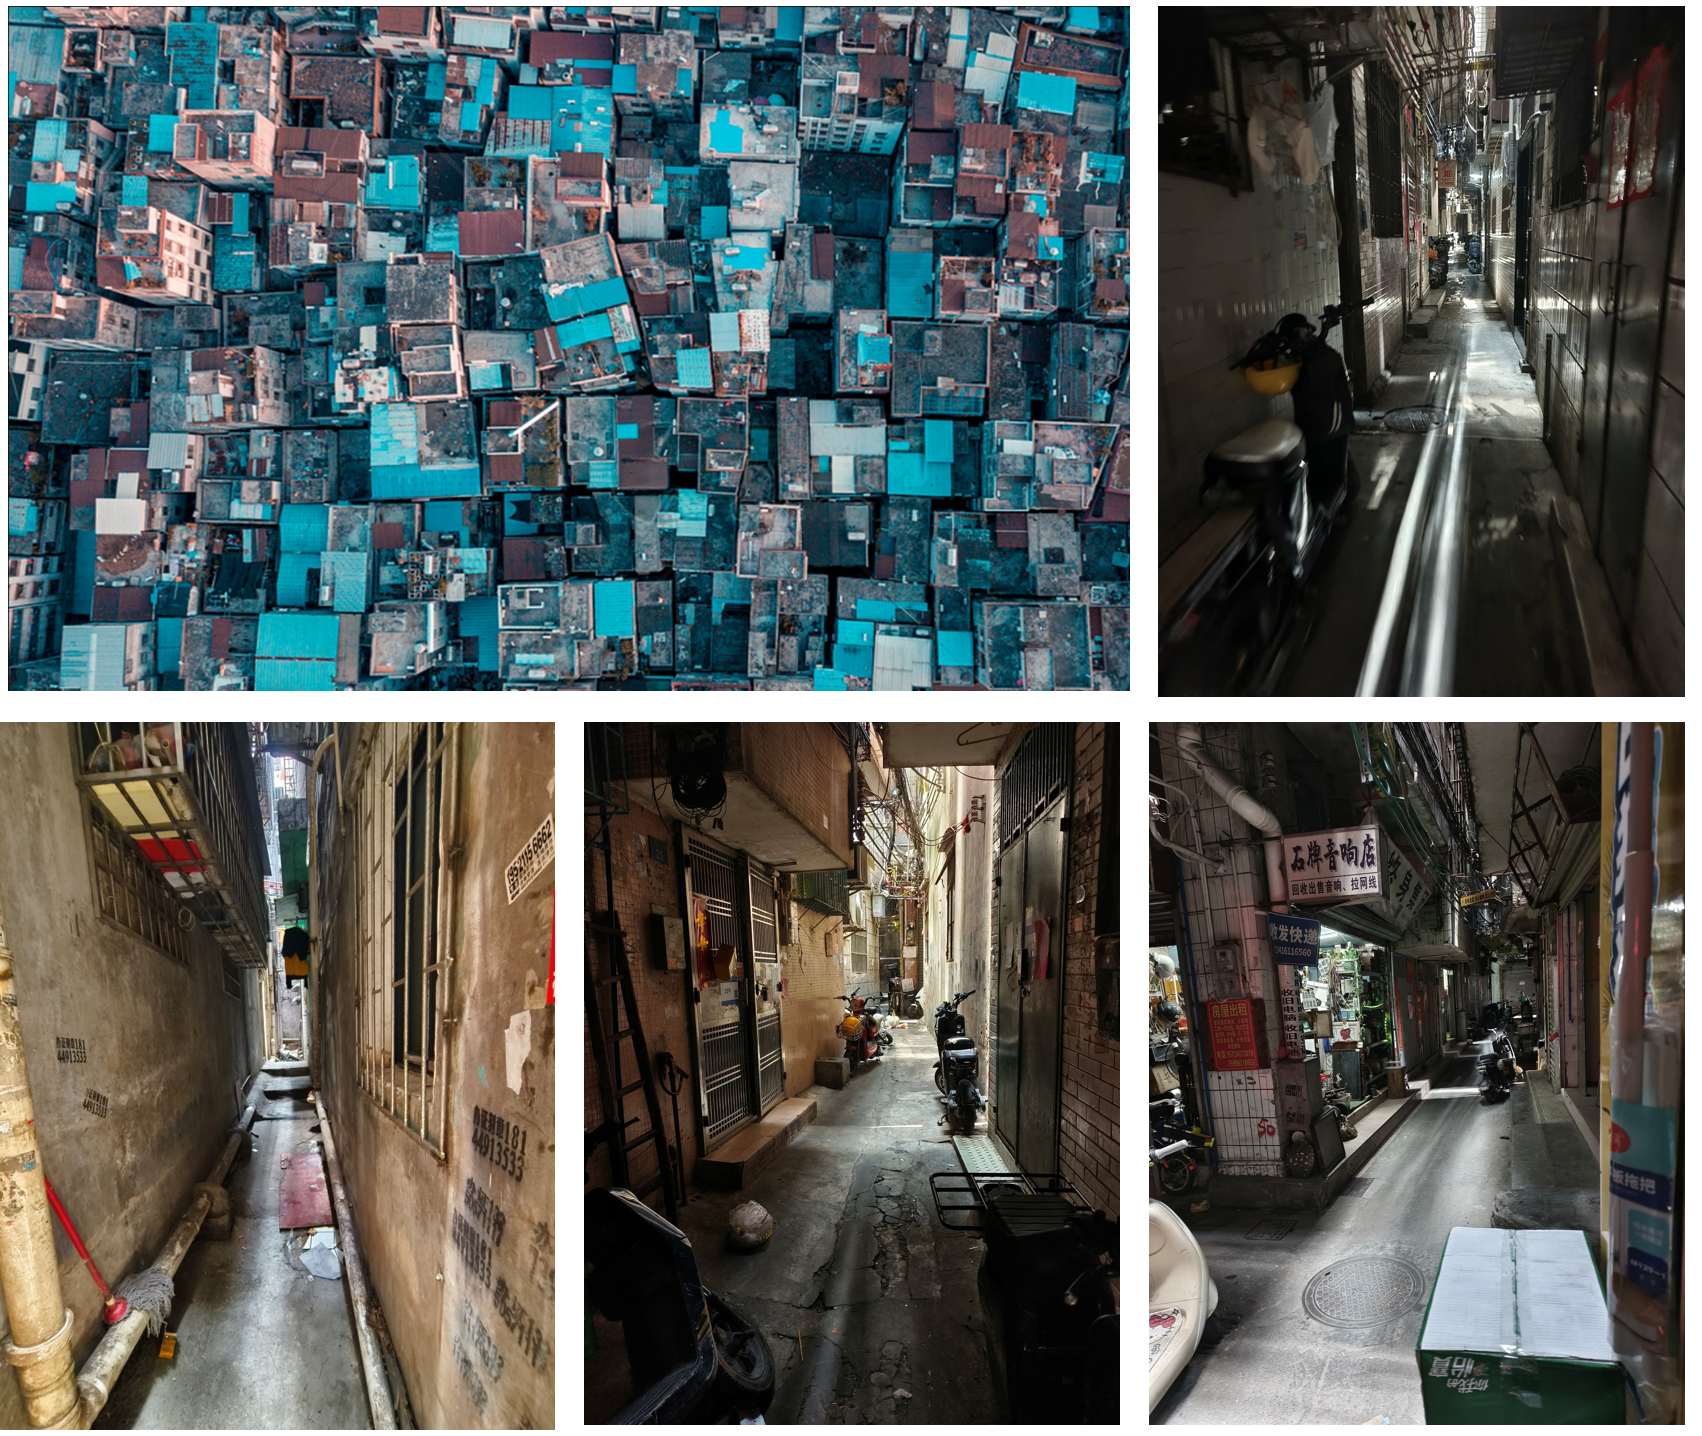
\includegraphics[width=0.75\linewidth]{fig/shipai_street_view.png}
    \caption{Aerial and street views of typical urban informal settlements in southern China, characterized by dense buildings and populations, narrow alleys, and intricate road networks, which collectively pose significant safety risks.}
    \label{fig:example}
\end{figure}


With rapid urbanization, informal settlements emerge worldwide under poorly planned conditions and inadequate living environments \citep{un-habitat2004}. The United Nations' Sustainable Development Goal 11 (SDG 11) calls for the creation of sustainable and inclusive cities, emphasizing the upgrading of informal settlements to ensure adequate, safe and affordable housing \citep{unitednations2015transforming,tu2024towards}. In China, informal settlements are primarily manifested as urban villages in cities, which are formed when formerly rural settlements are engulfed by expanding cities while retaining collectively owned land, informal construction patterns, and hybrid governance arrangements \citep{cao2025mapping,Wu2013UrbanVillagesInformality}.
In many southern megacities, these settlements provide large amounts of affordable rental housing and support intense daily mobility, yet their built form is often characterized by extremely high building density, fine-grained parcels, and labyrinthine alley systems \citep{Liu2010UrbanVillages,Lin2011VillageCity}, as shown in Figure \ref{fig:example}.
These dense and poorly connected morphologies can increase fire risk and hinder emergency response: narrow alleys can be impassable to fire engines and delay firefighting access \citep{Tang2010UrbanVillageFire,ChenEtAl2019NarrowAlleys}. Under demand for evacuation, restricted passages can also intensify crowd congestion and bottleneck effects \citep{Helbing2000Panic,Helbing2007CrowdDisasters}.



Conventional renewal policies that rely on large-scale demolition and reconstruction have become increasingly difficult to implement in urban villages due to high financial costs, complicated property-right structures, and stakeholder conflicts \citep{zhang2025mapping,Hao2011UrbanVillagesShenzhen}.
Urban-village renewal has often taken the form of comprehensive demolition and reconstruction; the Liede project, for example, was a wholesale redevelopment of the entire village \citep{LiEtAl2014LiedeUrbanPolicy}. More recently, \emph{micro-regeneration} (or micro-renewal) has emerged as a smaller-scale and participatory approach that seeks to improve existing neighborhoods while limiting wholesale demolition \citep{Wang2024MicroRegeneration,Zhu2023MicroRegeneration}.
Representative micro-regeneration studies have focused on heritage, public-space design, governance, and stakeholder participation rather than evacuation outcomes \citep{Wang2024MicroRegeneration,Zhu2023MicroRegeneration}. This study addresses a narrower question: how meter-scale geometric interventions affect simulated evacuation performance.
Urban-village streets are typically fine-grained and spatially complex \citep{Liu2010UrbanVillages,cao2025mapping}. At the same time, verification and validation of evacuation models are constrained by the availability of context-matched empirical data \citep{Ronchi2016VVEvacuationModels}. For the present planning problem, these two conditions complicate the benefit-based prioritization of local interventions.
The irregular, narrow geometry can also produce nonlinear crowd phenomena, including stop-and-go waves, arching at exits, and congestion at bottlenecks \citep{Helbing2000Panic,Helbing2007CrowdDisasters}. Extrapolating such local interactions to settlement-scale performance therefore requires an explicit dynamic model.

In this study, we frame micro-regeneration planning as a constrained multi-objective evacuation-design problem in which evacuation performance and reconstruction cost are evaluated jointly.
Multi-objective evolutionary algorithms have been applied to evacuation planning that jointly considers routes and safe-area allocation \citep{Saadatseresht2009MOEA,yang2025}; Particle Swarm Optimization method has also been explored in pedestrian evacuation modeling and obstacle-layout optimization \citep{Zheng2012PSOEvacuation,CristianiPeri2017Obstacles}. These methods are attractive when objectives conflict and the design variables are discrete or simulation-based \citep{Deb2002NSGA2}.
Many network-based evacuation optimization models operate at a macroscopic or dynamic-network-flow level, representing movement through link or edge capacities and travel times \citep{Bayram2016EvacuationReview,AalamiKattan2020}. Such abstractions are useful for regional planning but do not directly resolve meter-scale alley widths, local turns, and pedestrian interactions.
Therefore, a key unresolved question is how to translate micro-scale geometric interventions into a rigorous optimization design space while evaluating their system-level impacts through behavior-aware evacuation dynamics.

Quantitative decision support for micro-regeneration therefore requires two complementary capabilities.
First, it needs to reconstruct the environment at sufficient spatial fidelity (e.g., alley widths, turning constraints, dead-ends, porous connectivity) and represent global guidance toward exits under complex topology \citep{CovaChurch1997EvacuationGIS,Khatib1986PotentialField,Dijkstra1959,Sethian1996FastMarching}.
Second, it is necessary to capture the mobility of the crowd under emergency conditions, where local interactions and density effects dominate system performance \citep{Helbing1995SocialForce,Hughes2002ContinuumPedestrians,Treuille2006ContinuumCrowds}.
Although there are numerous evacuation models, verification and validation are widely recognized as challenging due to limited datasets of real-world evacuation, heterogeneous behaviors, and scenario-specific uncertainties, a limitation that is especially salient in informal settlements where high-quality monitoring data is scarce \citep{Ronchi2016VVEvacuationModels}.
These issues motivate simulation approaches that couple high-resolution spatial representations with scalable crowd dynamics, and that can be systematically calibrated and stress-tested.

Simulation--optimization can couple microscopic pedestrian models with optimization. CellEVAC, for example, integrates a Social Force simulation with behavioral exit-choice optimization and evaluates the system in a simulated Madrid Arena scenario \citep{LopezCarmonaGarcia2021CellEVAC}. Neither that study nor the hazard-specific route-planning study of \cite{yang2025} addresses physical micro-regeneration in irregular urban-village street networks. This leaves a specific methodological gap between simulation diagnostics and actionable spatial interventions.

Road networks can be represented as spatial graphs, and centrality measures can characterize structurally prominent streets or junctions \citep{Crucitti2006CentralityStreets}. In particular, betweenness centrality measures the extent to which a node or edge lies on shortest paths and can be computed efficiently using the algorithm of \cite{Brandes2001Betweenness}. These structural indicators may help screen candidate bottlenecks, but they do not by themselves establish time-dependent evacuation congestion \citep{Helbing2000Panic,Hughes2002ContinuumPedestrians}.
To bridge network structure and dynamic performance, microscopic and continuum crowd models (e.g., Social Force, cellular automata, SPH-based methods) have been used to reproduce key crowd phenomena such as congestion waves and capacity drops \citep{DANG2024102955}.
Among them, Smoothed Particle Hydrodynamics (SPH), as a meshfree Lagrangian approach, has shown promise for dense crowds due to numerical robustness and its natural representation of continuous density evolution and complex boundaries \citep{Yuan2020SPHPedestrianFlow,DANG2024102955}.
At the building scale, pedestrian simulation has also been used to compare candidate exit-door locations and evacuation-area designs \citep{muhammed2020simulation}. Such studies do not directly address settlement-scale physical interventions in irregular outdoor street networks.

Building on these foundations, this paper proposes a coupled \emph{simulation--optimization} framework to support micro-regeneration decisions in dense urban informal settlements.
We (i) reconstruct a GIS-based environment and compute a navigation field toward exits to provide consistent global guidance in irregular networks,
(ii) simulate emergency crowd mobility with an SPH-informed crowd-density and interaction model to capture congestion formation and dissipation,
and (iii) search for cost-effective intervention portfolios using a multi-objective evolutionary algorithm, explicitly trading off evacuation efficiency and reconstruction cost.
A case study of Shipai Village in Guangzhou, China illustrates how the framework can identify a small set of bottlenecks where minor geometric modifications yield substantial evacuation-time reductions.

In summary, our main contributions are threefold:
\begin{itemize}
  \item We propose a coupled simulation-optimization framework that can assess and enhance the performance of road networks during dynamic disaster evacuation in dense urban informal settlements. This framework supports evidence-based micro-regeneration by bridging the gap between simulation diagnostics and actionable interventions, and it holds broader applicability to other high-density urban environments. 
  \item We develop a multi-objective optimization pipeline that formalizes urban micro-regeneration as a discrete intervention design space and automatically identifies high benefit–cost portfolios (balancing evacuation time and reconstruction cost), enabling transparent trade-off analysis.
  \item We validate the proposed method through extensive experiments in Shipai Village—a famous and typical urban informal settlement in Guangzhou characterized by extremely high population and building density and an intricate, irregular road network—demonstrating the framework’s effectiveness and practical relevance.
\end{itemize}

\revb{The remainder of this paper is organized as follows.
Section~\ref{sec:method} introduces the proposed simulation--optimization framework.
Section~\ref{sec:calibration_validation} presents movement-model calibration and corridor-scale validation.
Section~\ref{sec:experiments} reports the Shipai Village case study, including baseline diagnosis, road-network
optimization, case-scale verification, sensitivity analysis, and computational performance.
Section~\ref{sec:discussion_revised} discusses applicability and limitations, and
Section~\ref{sec:conclusion} concludes the paper.}

\section{Methodology}
\label{sec:method}

\begin{sloppypar}
This section presents the computational framework developed to evaluate evacuation performance in high-density environments of urban informal settlements. As shown in Figure~\ref{fig:framework}, the framework consists of three integrated components: (1) computational environment construction, (2) crowd evacuation simulation, and (3) optimization of road-network interventions. 
Through the integration of these three components, the framework provides cost-effective micro-scale retrofit strategies for urban informal settlements and offers a quantitative basis for decision making in sustainable urban development.
Details of the components are elaborated in the following subsections.
\end{sloppypar}

\begin{figure}[h]
    \centering
    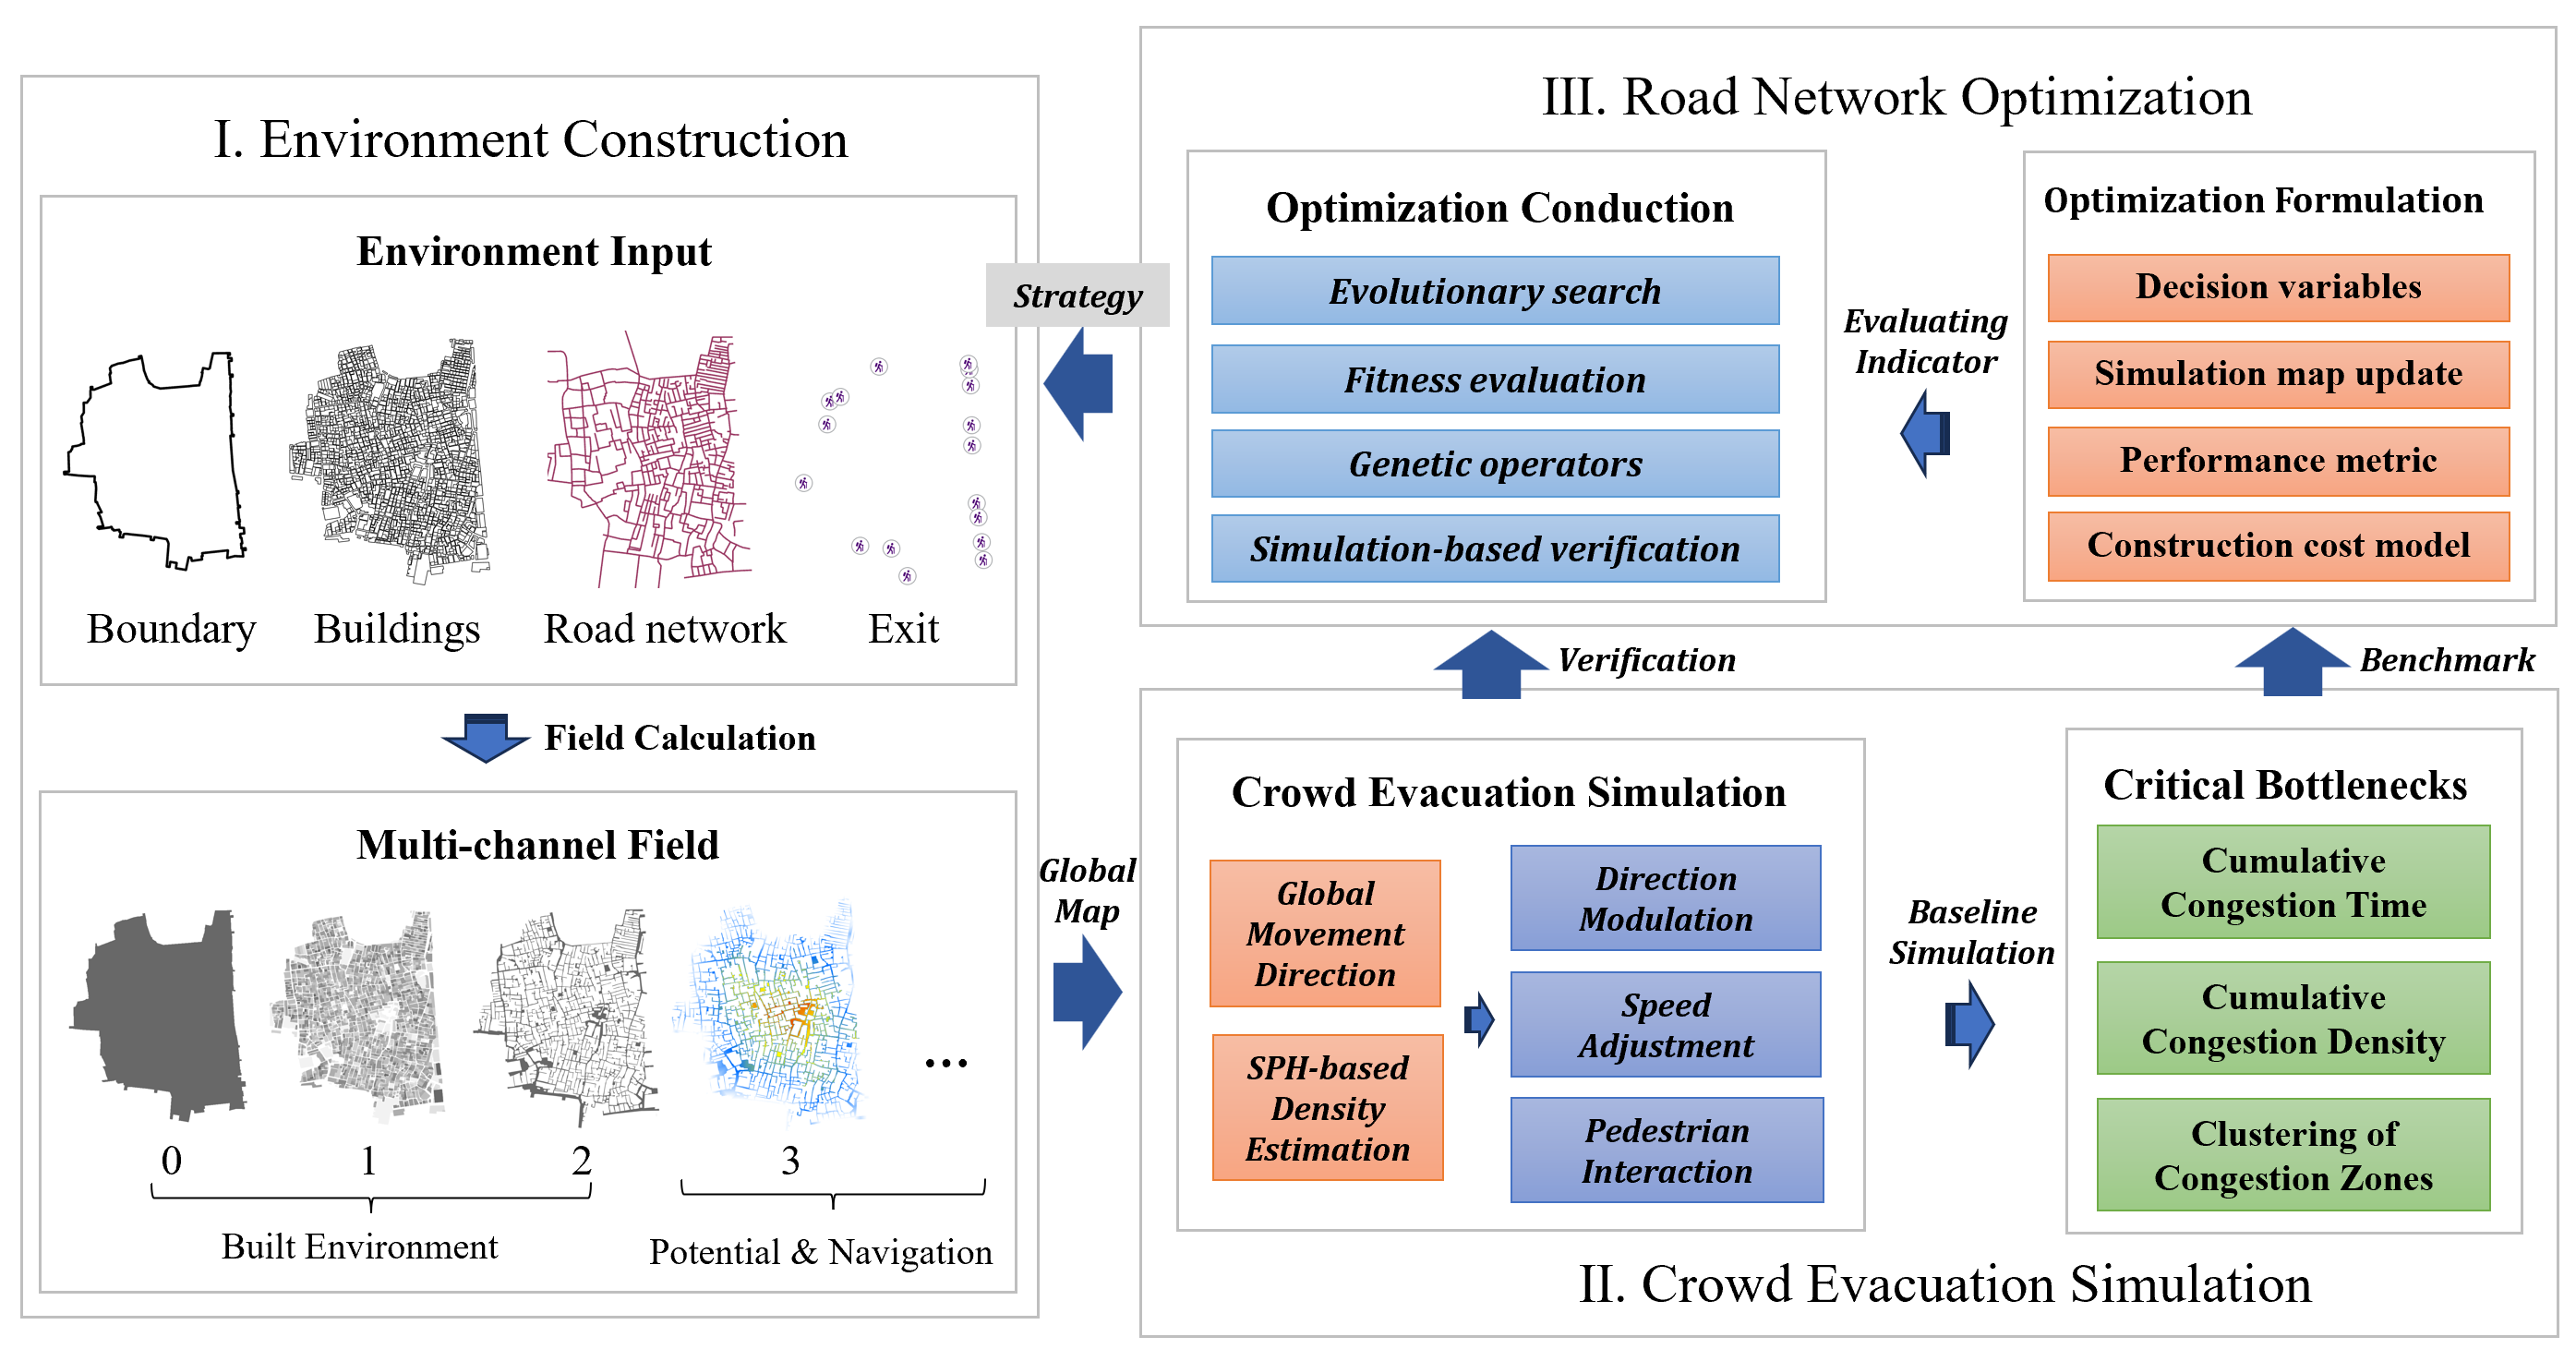
\includegraphics[width=1\linewidth]{fig/framework.png}
    \caption{Overview of the proposed simulation–optimization framework. It consists of three integrated components: (1) computational environment construction, (2) crowd evacuation simulation modeling, and (3) road network optimization.}
    \label{fig:framework}
\end{figure}


\subsection{Computational Environment Construction}
\label{sec:env}


We first construct a multi-channel grid representation of the dense environment from
high-resolution GIS data. This rasterized environment explicitly encodes walkability, corridor
widths, obstacles/buildings, and exit locations on a unified raster domain, providing a consistent
spatial substrate for both field computation and agent-based simulation. We then compute a road-network potential field to generate a \emph{global navigation direction field} (as illustrated in Figure \ref{fig:globalnavigation}),
which serves as the baseline guidance prior to introducing any density- or hazard-dependent
feedback.

% \paragraph{Multi-channel rasterization.}
To handle the highly fragmented alley topology in urban informal settlements, we convert GIS layers
(including buildings, boundaries, roads, and exits) into a high-resolution raster map with spatial
resolution $r=0.1$\,m. Each cell stores multiple channels, including a walkable mask
$\Omega_{\mathrm{walk}}$, an obstacle/building mask $\Omega_{\mathrm{obs}}$, an exit mask
$\Omega_{\mathrm{exit}}\subset\Omega_{\mathrm{walk}}$, and optional geometric attributes such as local
corridor width (estimated by distance-to-obstacle or medial-axis style operators). This
representation preserves fine-scale connectivity (narrow alleys, dead-ends, and sharp turns) and
enables neighborhood-based computation on the same discretization used in simulation.

% \paragraph{Static distance potential (no density feedback).}
On the walkable domain $\Omega_{\mathrm{walk}}$, we compute an exit-to-cell distance potential
$\Phi(\mathbf{x})$ using multi-source Dijkstra search on the weighted walkable graph induced by the
8-neighborhood $\mathcal{N}_8(\mathbf{x})$. All exit cells are initialized as zero-distance sources:
\begin{equation}
\Phi(\mathbf{x})=
\begin{cases}
0, & \mathbf{x}\in\Omega_{\mathrm{exit}},\\
\min_{\mathbf{y}\in\mathcal{N}_8(\mathbf{x})}\{\Phi(\mathbf{y})+w(\mathbf{x},\mathbf{y})\}, & \mathbf{x}\in\Omega_{\mathrm{walk}},\\
+\infty, & \text{otherwise},
\end{cases}
\label{eq:potential-dijkstra}
\end{equation}
where the fixed geometric edge cost is
\begin{equation}
w(\mathbf{x},\mathbf{y})=
\begin{cases}
r, & \text{for an axial move},\\
\sqrt{2}\,r, & \text{for a diagonal move}.
\end{cases}
\end{equation}
Because all edge costs are non-negative, multi-source Dijkstra search with a minimum-priority queue
produces the exact shortest-path distance on the weighted raster graph. Obstacles are impassable and
therefore excluded from the search.



% \paragraph{Global navigation direction field.}
The distance potential $\Phi(\mathbf{x})$ defines a globally consistent \emph{static} shortest-path
structure to the nearest exit on the raster graph. We convert this scalar potential into a
direction field by taking the negative normalized gradient:
\begin{equation}
\mathbf{d}_{\mathrm{nav}}(\mathbf{x})
= -\frac{\nabla \Phi(\mathbf{x})}{\|\nabla \Phi(\mathbf{x})\|+\epsilon},
\label{eq:nav-gradient}
\end{equation}
where $\epsilon$ is a small constant for numerical stability in near-flat regions. In practice, we
compute $\nabla \Phi$ by finite differences on the grid (e.g., central differences where available
and one-sided differences near obstacles/boundaries), and we evaluate $\mathbf{d}_{\mathrm{nav}}$ only
on $\Omega_{\mathrm{walk}}$. Intuitively, $\mathbf{d}_{\mathrm{nav}}(\mathbf{x})$ acts as a ``compass''
vector pointing toward the locally steepest descent direction of the exit-distance map; following
this field yields a shortest-path-like route under the chosen local cost $w(\cdot)$, while remaining
globally coherent across the maze-like corridor network.
The construction of the multi-source Dijkstra distance field and the resulting gradient-based navigation directions are illustrated in Figure~\ref{fig:globalnavigation}.



% \paragraph{Discussion of scope.}
We emphasize that this global field is \emph{purely geometric} and time-invariant: it encodes
shortest paths to exits under fixed traversal costs and does not react to evolving crowd density,
queueing, or hazards. As such, it provides a clean baseline guidance layer that captures the
connectivity constraints of ultra-narrow alleys, and it also serves as the reference field for
subsequent extensions that incorporate dynamic density- or hazard-dependent costs in later sections.
\begin{figure}
    \centering
    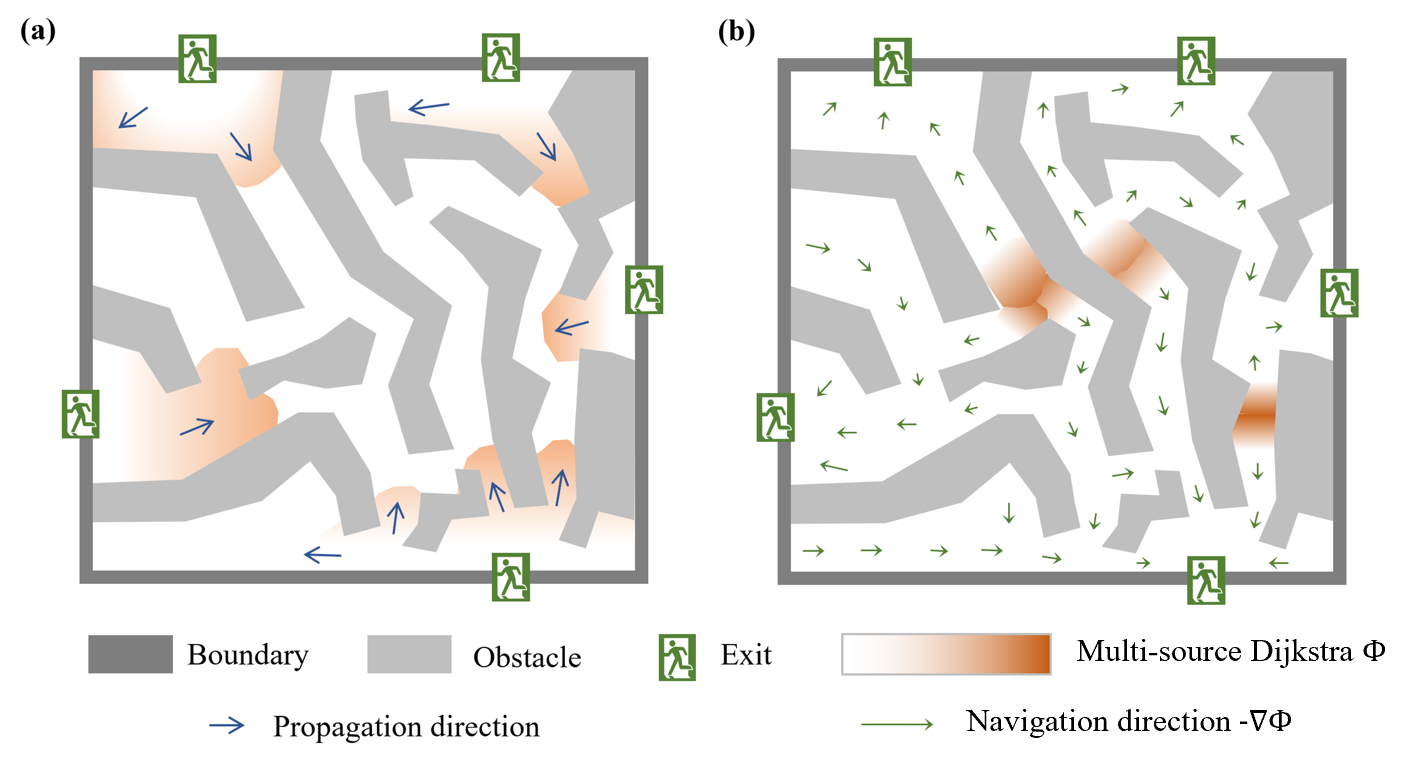
\includegraphics[width=0.80\linewidth]{fig/BFS.png}
    \caption{Illustration of the distance-to-exit field and the derived navigation field. (a) Multi-source Dijkstra search computes the obstacle-aware weighted distance-to-exit field on the walkable raster, where all exits are treated as sources. (b) The global navigation field is obtained by taking the negative spatial gradient of the distance field, producing local guidance directions that lead agents toward the nearest exit along feasible corridors.}
    \label{fig:globalnavigation}
\end{figure}
% \FloatBarrier

% ------------------------------------------------
\subsection{Crowd Evacuation Simulation Modeling}
\label{sec:movingmodel}

Given the multi-channel grid environment, each pedestrian is guided by a precomputed global navigation direction field that provides a desired moving direction toward exits, similar to a ``compass'' defined for every walkable cell (as illustrated in Figure \ref{fig:globalnavigation}). 
At runtime, pedestrians do not strictly follow this direction: they continuously adjust their velocity in response to nearby neighbors and obstacles, so that local collision avoidance, queueing, and lane formation can emerge naturally in dense regions.

To model these local interactions in a continuous and stable manner, we adopt a Smoothed Particle Hydrodynamics (SPH)-style formulation \citep{vanToll2021SPHCrowds, Yuan2020SPHPedestrianFlow}, where each pedestrian is treated as a particle carrying position and velocity. 
%
Neighbor influence is aggregated through a compact-support kernel within a finite interaction radius, producing density/pressure-like terms (for personal-space preservation) and viscosity-like terms (for velocity smoothing and damping), which together yield realistic congestion effects without hand-crafted rules for overtaking or stopping.
%
The simulator outputs full trajectories and time-resolved crowd fields (e.g., density and congestion time), enabling post-hoc identification of recurrent bottlenecks and hazard-exposure zones by locating cells with persistent high density, long dwell time, or high accumulated risk.


% \paragraph{Density and pressure.}
For pedestrian $i$ at position $\mathbf{x}_i$, the local crowd density is estimated using an SPH kernel:
\begin{equation}
\rho_i=\sum_{j} m_j\,W(\|\mathbf{x}_i-\mathbf{x}_j\|,h),
\label{eq:sph-density_s}
\end{equation}
where $m_j$ is the agent weight and $W(\cdot)$ is a Gaussian kernel truncated at $r\le 3h$.
Density is converted to a congestion pressure via a linear equation of state:
\begin{equation}
P_i = k \, (\rho_i - \rho_0),
\label{eq:pressure_s}
\end{equation}
where $\rho_0$ is the preferred (uncongested) density and $k$ controls compressibility.

% \paragraph{Local interaction and local direction.}
Neighbor-induced repulsion is driven by the pressure gradient:
\begin{equation}
\mathbf{f}_i^{\mathrm{int}}
=
- \sum_{j}
m_j
\left(
\frac{P_i}{\rho_i^2}
+
\frac{P_j}{\rho_j^2}
\right)
\nabla W(\|\mathbf{x}_i - \mathbf{x}_j\|, h).
\label{eq:interaction_s}
\end{equation}
We define the \emph{local interaction direction} as the normalized resultant force
(with a small $\varepsilon$ for numerical stability):
\begin{equation}
\mathbf{l}_i = \frac{\mathbf{f}_i^{\mathrm{int}}}{\|\mathbf{f}_i^{\mathrm{int}}\|+\varepsilon}.
\label{eq:local_dir_s}
\end{equation}
This $\mathbf{l}_i$ summarizes short-range avoidance and lateral bypass tendencies in a unified form,
and becomes dominant only in dense regions.

% \paragraph{Navigation--interaction coupling and state update.}
Let $\mathbf{g}_i=\mathbf{d}_{\mathrm{nav}}(\mathbf{x}_i)$ denote the global navigation direction.
We blend global and local directions using a density-adaptive weight:
\begin{equation}
\mathbf{d}_i=(1-\alpha_i)\mathbf{g}_i+\alpha_i\mathbf{l}_i,\qquad
\alpha_i=\mathrm{clip}\!\left(\frac{\rho_i-\rho_{\mathrm{low}}}{\rho_{\mathrm{high}}-\rho_{\mathrm{low}}},0,1\right).
\label{eq:dir-blend_s}
\end{equation}
The desired speed follows a calibrated exponential fundamental diagram:
\begin{equation}
v_i=v_f \exp\!\left[-\left(\frac{\rho_i}{\rho_0}\right)^{n}\right],
\label{eq:speed_underwood_s}
\end{equation}
and the discrete-time update is
\begin{equation}
\mathbf{v}_i=v_i\frac{\mathbf{d}_i}{\|\mathbf{d}_i\|+\varepsilon},\qquad
\mathbf{x}_i(t+\Delta t)=\mathbf{x}_i(t)+\mathbf{v}_i(t)\Delta t.
\label{eq:state-update_s}
\end{equation}


\subsection{Targeted Micro-Regeneration for Road-Network Improvement}
\label{sec:method_micro_regen}

To improve evacuation efficiency under strict spatial and construction constraints, we perform
\emph{targeted micro-regeneration} by widening only a small set of simulation-identified bottlenecks.
Our pipeline includes: (i) bottleneck identification from the baseline simulation,
(ii) discrete decision formulation with simulation-in-the-loop objectives,
and (iii) evolutionary optimization with verification.

\subsubsection{Phase I: Bottleneck Identification from Baseline Simulation}
\label{sec:method_bottleneck}

% We run a baseline SPH evacuation simulation on the initial build environment.
% Let $\rho(\mathbf{p},t)$ and $v(\mathbf{p},t)$ denote the density and mean speed at raster cell
% $\mathbf{p}$ and time $t$. We characterize persistent congestion using two complementary measures.

The baseline simulation is sampled at discrete times $\{t_n\}_{n=1}^{N}$ with a fixed step size $\Delta t$,
so that $T = N\Delta t$ is the total observation horizon.
Let $\mathcal{A}_{\mathbf{p}}(t_n)$ be the set of active pedestrians assigned to raster cell $\mathbf{p}$ at time $t_n$,
and let $v_i(t_n)$ and $\rho_i(t_n)$ denote the speed and SPH density of pedestrian $i$, respectively.

First, Cumulative Congestion Time (CCT) is used to describe the low-speed persistence: 

\begin{equation}
T_{\mathrm{cong}}(\mathbf{p})
=\sum_{n=1}^{N}\sum_{i\in\mathcal{A}_{\mathbf{p}}(t_n)}
\mathbb{I}\!\left(v_i(t_n)<v_{\mathrm{th}}\right)\Delta t ,
\label{eq:tcong}
\end{equation}
where $v_{\mathrm{th}}$ is the speed threshold that defines a ``congested'' (low-mobility) state,
and $T_{\mathrm{cong}}(\mathbf{p})$ accumulates the low-speed pedestrian--time exposure in that cell.
The indicator function $\mathbb{I}(\cdot)$ equals $1$ if the condition holds and $0$ otherwise.

Second, Cumulative Crowd Density (CCD) is used to describe cumulative density exposure:
\begin{equation}
D_{\mathrm{cum}}(\mathbf{p})
=\sum_{n=1}^{N}\sum_{i\in\mathcal{A}_{\mathbf{p}}(t_n)}
\rho_i(t_n)\Delta t ,
\label{eq:rhocong}
\end{equation}
where each active pedestrian contributes its SPH density over the time step $\Delta t$;
no instantaneous density threshold or conditional averaging is applied.



Cells are marked as candidates if they are simultaneously ``time-congested'' and ``density-congested'':
\begin{equation}
\mathbb{I}_{\mathrm{cand}}(\mathbf{p})
=
\mathbb{I}\!\left(T_{\mathrm{cong}}(\mathbf{p})\ge T_{\mathrm{th}}\right)
\wedge
\mathbb{I}\!\left(D_{\mathrm{cum}}(\mathbf{p})\ge D_{\mathrm{th}}\right).
\label{eq:candmask}
\end{equation}
Eq.~\eqref{eq:candmask} marks a cell as a candidate bottleneck only if it is both
\emph{persistent} in low speed and subject to high cumulative density exposure.
In practice, $(v_{\mathrm{th}}, T_{\mathrm{th}}, D_{\mathrm{th}})$
can be chosen in three common ways:
(i) domain-informed values,
(ii) percentile-based thresholds for the cumulative fields,
or (iii) calibrated values that maximize agreement with visually identified bottlenecks
in the baseline simulation snapshots.

% The set of candidate congested cells $\Omega=\{\mathbf{p}\mid \mathbb{I}_{\mathrm{cand}}(\mathbf{p})=1\}$
% is clustered (DBSCAN) into $K$ spatial zones $\mathcal{Z}=\{z_1,\ldots,z_K\}$.
% Each zone is then mapped to one representative road bottleneck segment, yielding
% $\mathcal{E}=\{e_1,\ldots,e_K\}$.

% \paragraph{\textbf{Spatial clustering and mapping to bottleneck segments}}
The candidate set $\Omega=\{\mathbf{p}\mid \mathbb{I}_{\mathrm{cand}}(\mathbf{p})=1\}$ is spatially clustered by DBSCAN \citep{ester1996density}.
DBSCAN is a density-based clustering algorithm widely used in machine learning, which is capable of discovering clusters of arbitrary shape. It requires two parameters: the neighborhood radius $\epsilon_{\mathrm{db}}$ (in meters or cells),
and the minimum number of points $m_{\mathrm{db}}$ to form a cluster.
We set $\epsilon_{\mathrm{db}}$ to match the expected geometric width of local congestion patches
(e.g., comparable to alley width under the raster resolution), and $m_{\mathrm{db}}$ to suppress isolated noisy cells.
The resulting clusters correspond to $K$ congestion zones $\mathcal{Z}=\{z_1,\ldots,z_K\}$.
Each zone $z_k$ is then mapped to a representative road bottleneck segment $e_k$ by projecting
the cluster cells onto the walkable-network skeleton (or centerline) and selecting the shortest
cross-section / narrowest local passage intersecting the cluster,
yielding the bottleneck set $\mathcal{E}=\{e_1,\ldots,e_K\}$ for subsequent interventions.


\subsubsection{Phase II: Discrete Formulation and Simulation-in-the-Loop Objectives}
\label{sec:method_formulation}
% \paragraph{From Phase I to Phase II.}
Phase~I yields a set of representative bottleneck segments
$\mathcal{E}=\{e_1,\ldots,e_K\}$ by clustering candidate congested cells and projecting each cluster onto the walkable network.
Phase~II treats these $K$ bottlenecks as \emph{discrete intervention sites} and searches for a widening scheme
that balances evacuation efficiency and a raster-based demolition/land-take proxy under a consistent representation.

% \paragraph{Discrete widening decisions and feasibility.}
% \paragraph{Discrete widening decisions.}
A widening scheme is encoded as a discrete decision vector:
\begin{equation}
\boldsymbol{x}=[\delta_1,\ldots,\delta_K]\in\mathcal{D}^K,\qquad
\delta_k\in\mathcal{D}=\{0,2,4\}\ (\mathrm{m}),
\label{eq:decision}
\end{equation}
where $\delta_k$ is the added width assigned to segment $e_k$.
The discrete set $\mathcal{D}=\{0,2,4\}$\,m reflects practical engineering choices (no change / moderate / strong widening),
and also keeps the search space finite and interpretable.
Note that $\delta_k=0$ means bottleneck $e_k$ is left unchanged.

% \paragraph{Deterministic map update and simulator evaluation.}
Given $\boldsymbol{x}$, we modify the raster environment through a deterministic operator $\mathcal{M}(\cdot)$
that expands the walkable region around each target segment according to $\delta_k$ while respecting the obstacle/building masks.
This produces an updated multi-channel raster map (with the same resolution $r$ as in Phase~I).
We then evaluate the modified map by running a full SPH evacuation simulation $\mathcal{S}(\cdot)$
under \emph{identical} initial conditions (population size, initial positions, desired-speed distribution, exits, and time step).

Then, the simulation-in-the-loop pipeline can be formulated as follows: 
\begin{equation}
\text{outputs } \big(A_{\boldsymbol{x}}(t),\ N_{\mathrm{grid}}(\boldsymbol{x}),\ldots\big)
= \mathcal{S}\!\big(\mathcal{M}(\boldsymbol{x})\big),
\label{eq:simloop}
\end{equation}
returning:
(i) the residual population curve $A_{\boldsymbol{x}}(t)$, i.e., the number of agents remaining inside the domain at time $t$,
\revb{and (ii) $N_{\mathrm{grid}}(\boldsymbol{x})$, the number of building cells occupied by the widened road under $\mathcal{M}(\boldsymbol{x})$,
which provides the raster basis for estimating reconstruction cost rather than a complete monetary estimate.}


% \paragraph{Evacuation performance objective.}
Let $t_{\mathrm{start}}$ be the evacuation start time (typically $0$) and let $t_{\mathrm{end}}$ be the completion time,
defined as the first time when all agents have exited (or when $A_{\boldsymbol{x}}(t)$ reaches a small tolerance).
We denote the corresponding clearance duration by $T(\boldsymbol{x})=t_{\mathrm{end}}-t_{\mathrm{start}}$ and define a normalized residual-population integral:
\begin{equation}
\eta(\boldsymbol{x})=
\frac{1}{A(t_{\mathrm{start}})\,T(\boldsymbol{x})}
\int_{t_{\mathrm{start}}}^{t_{\mathrm{end}}}A_{\boldsymbol{x}}(t)\,\mathrm{d}t.
\label{eq:eta}
\end{equation}

Beyond clearance time, we also penalize scenarios where a large fraction of the population remains inside the domain for long periods.
To that end, Eq.~\eqref{eq:eta} defines a normalized residual-population integral
\(\eta(\boldsymbol{x})\in[0,1]\), where $A(t_{\mathrm{start}})$ is the initial population size. Intuitively, $\eta(\boldsymbol{x})$ is the \emph{average normalized residual fraction} during evacuation;
smaller values indicate faster depletion of the crowd. 

Then, we compute the evacuation objective as: 
\begin{equation}
F_{\mathrm{evac}}(\boldsymbol{x}) = T(\boldsymbol{x})\Big(1+\alpha\,\eta(\boldsymbol{x})\Big),
\label{eq:fevac}
\end{equation}
% which penalizes both long clearance time and persistently high residual crowding.

where the clearance time $T(\boldsymbol{x})$ serves as the baseline objective, while the factor $1+\alpha\,\eta(\boldsymbol{x})$ imposes an additional penalty for persistent residual crowding. The parameter $\alpha\geq 0$ controls the strength of this penalty. When $\alpha=0$, the objective reduces to minimizing the clearance time alone.

To compare the implementation burden of different widening patterns, we estimate
reconstruction cost on a raster-consistent basis. Let $r$ denote the raster cell
size (meters per cell); each building cell occupied by the widened road corresponds
to an affected area $r^2$. The reconstruction cost is defined as:
\begin{equation}
F_{\mathrm{cost}}(\boldsymbol{x})
=
c \cdot N_{\mathrm{grid}}(\boldsymbol{x})\,r^2 ,
\label{eq:fcost}
\end{equation}
where $N_{\mathrm{grid}}(\boldsymbol{x})$ is the number of affected building cells,
$r^2$ is the area represented by each cell, and $c$ is the unit reconstruction-cost
coefficient per square meter. Because $c$ is expressed in relative units,
$F_{\mathrm{cost}}$ provides a consistent comparative estimate rather than a
complete monetary valuation. Applying the same definition to all candidate schemes
ensures a consistent basis for cost comparison.

% \paragraph{Bi-objective problem statement.}
Finally, Phase~II formulates targeted micro-regeneration as the bi-objective optimization:

% \paragraph{Bi-objective micro-regeneration problem.}
% The targeted widening problem is formulated as
\begin{equation}
\min_{\boldsymbol{x}\in\mathcal{D}^K}\ \Big(F_{\mathrm{evac}}(\boldsymbol{x}),\ F_{\mathrm{cost}}(\boldsymbol{x})\Big).
\label{eq:biobj}
\end{equation}
%
We seek expansion schemes $\boldsymbol{x}\in\mathcal{D}^K$ that jointly minimize evacuation loss
$F_{\mathrm{evac}}(\boldsymbol{x})$ and the reconstruction cost $F_{\mathrm{cost}}(\boldsymbol{x})$. Here, the reconstruction cost encompasses demolition, construction, land acquisition, and compensation expenses.

Since each evaluation requires a full SPH simulation (Eq.~\eqref{eq:simloop}) and the decision space is discrete,
we adopt an evolutionary search strategy in Phase~III.


\subsubsection{Phase III: Evolutionary Optimization and Verification}
\label{sec:method_optimization_overview}

\revb{We solve the micro-regeneration optimization problem (Eq.~\eqref{eq:biobj}) directly using a simulation-driven NSGA-II procedure}. Each individual corresponds
to a discrete widening scheme $\boldsymbol{x}\in\mathcal{D}^K$ and is evaluated by a full simulator run
(Eq.~\eqref{eq:simloop}). \revb{The two objective values are retained separately throughout selection; no fixed linear
weight is required to construct the nondominated solution set.} The overall procedure is summarized in
Algorithm~\ref{alg:ga}.


% \subsubsection{Phase III: Evolutionary Optimization and Verification}
% \label{sec:method_optimization_overview}

\begin{algorithm}[H]
\caption{Simulation-in-the-loop \textcolor{blue}{multi-objective NSGA-II} for discrete road widening}
\label{alg:ga}
\begin{algorithmic}[1]
\Require Candidate segments $\mathcal{E}=\{e_i\}_{i=1}^{K}$; discrete set $\mathcal{D}=\{0,2,4\}$;
population size $P$; offspring batches $G$; crossover probability $p_c$;
per-gene mutation probability $p_m$; penalty $F_{\mathrm{pen}}$.
\State Initialize population $\{\boldsymbol{x}^{(j)}\}_{j=1}^{P}$ with $\delta_i^{(j)} \sim \mathrm{Unif}(\mathcal{D})$
\State \revb{Include the no-intervention vector $\boldsymbol{0}$ as a reference individual}
\State \revb{Evaluate $\big(F_{\mathrm{evac}},F_{\mathrm{cost}}\big)$ for the initial population}
\For{$g=1$ to $G$}
  \State \revb{Rank parents by nondominated sorting and crowding distance}
  \State \revb{Select parents by binary tournament (rank first, crowding distance second)}
  \State Generate $P$ offspring by uniform crossover ($p_c$) and per-gene discrete mutation ($p_m$)
  \State \revb{Evaluate $\big(F_{\mathrm{evac}},F_{\mathrm{cost}}\big)$ for every offspring}
  \State \revb{Combine parents and offspring and retain $P$ individuals by rank and crowding distance}
  \State \revb{Compute fixed-reference Hypervolume from the unique rank-0 objective vectors}
\EndFor
\State \revb{\Return the final nondominated approximation $\widehat{\mathcal{P}}$}
\end{algorithmic}
\end{algorithm}

Specifically, Eq.~\eqref{eq:biobj} defines a discrete, simulation-based optimization problem: each candidate
$\boldsymbol{x}$ must be assessed by a full SPH run (Eq.~\eqref{eq:simloop}), which is expensive and non-differentiable.
We therefore adopt an evolutionary search that only requires objective evaluations and naturally handles discrete
decision variables.


% \paragraph{Preference interpretation after multi-objective optimization.}
\revb{For decision-support purposes, the two objectives can be summarized by the following scalar preference function:}
\begin{equation}
F(\boldsymbol{x}) = F_{\mathrm{evac}}(\boldsymbol{x})
+ \beta\,F_{\mathrm{cost}}(\boldsymbol{x}),
\label{eq:scalar_fitness}
\end{equation}
which provides the raster basis for estimating reconstruction cost rather than a complete monetary estimate.
The optimization itself is conducted in the original bi-objective space using NSGA-II, which retains
$F_{\mathrm{evac}}$ and $F_{\mathrm{cost}}$ as separate objectives rather than minimizing their weighted sum. This
formulation allows the search to approximate a diverse set of nondominated solutions without imposing a single
trade-off preference a priori. Equation~\eqref{eq:scalar_fitness} is subsequently applied as a post-optimization
decision criterion to identify a representative compromise solution from the approximated Pareto front under the
specified value of $\beta$. The no-intervention reference, reconstruction-cost-priority solution, ideal-point compromise solution,
and evacuation-priority solution are also reported to characterize the range of practically relevant trade-offs
available to decision makers.

\revb{Each candidate solution is encoded as a discrete vector
$\boldsymbol{x}=[\delta_1,\ldots,\delta_K]$, where $\delta_k\in\mathcal{D}$.
NSGA-II evolves these solutions through rank--crowding tournament selection,
uniform crossover with probability $p_c$, and per-gene discrete mutation with
probability $p_m$. Failed simulator runs are penalized in both objectives, while
the $(\mu+\lambda)$ environmental selection balances convergence toward the
nondominated set with diversity along the trade-off front. After $G$ offspring
batches, the unique nondominated solutions in the final population constitute
the finite-budget approximation of the Pareto front. Selected representative
solutions are then re-evaluated through $\mathcal{M}(\cdot)$ under identical
initial conditions and compared in terms of evacuation performance
($F_{\mathrm{evac}}$ and clearance time $T$), intervention cost
$F_{\mathrm{cost}}$, and the spatial dissipation of congestion characterized by
$T_{\mathrm{cong}}(\mathbf{p})$ and
$D_{\mathrm{cum}}(\mathbf{p})$ from Phase~I.}



% =======================================================
\section{Movement-Model Calibration and Validation}
\label{sec:calibration_validation}

\revb{The evaluation follows a hierarchical strategy that distinguishes component-level empirical validation from
case-scale verification. This section calibrates and validates the local pedestrian-movement dynamics against
corridor-level empirical evidence. Case-scale behavior is assessed separately after the study area, baseline
configuration, and representative intervention have been defined in Section~\ref{sec:experiments}. This separation is
important because agreement at the component level does not independently validate exit allocation, global navigation,
spatial congestion, or absolute settlement-scale clearance time.}

\subsection{Calibration and Validation Framework}
Our component-level evaluation focuses on the pedestrian fundamental diagram
\citep{flotterod2015bidirectionalFD}, which characterizes the relationships among density ($\rho$), speed ($v$), and
specific flow ($q$) in narrow corridors typical of urban informal settlements. Empirical studies consistently show that
walking speed decreases as density increases, while the corresponding flow is expressed as $q=\rho v$
\citep{seyfreid2005,zhangjun2013}. These relationships provide the empirical basis for calibrating the movement model and
for evaluating whether its simulated macroscopic response remains consistent with observed pedestrian dynamics.

We constructed a series of controlled simulation scenarios representing the narrow ``handshake'' alleys found in urban informal settlements in southern China (as illustrated in Figure \ref{fig:example}). The experimental settings are detailed in Table~\ref{tab:sim_settings}.

% Table: Simulation Settings
\begin{table}[htbp]
    \centering
    \caption{Experimental settings for micro-level model calibration and validation.}
    \label{tab:sim_settings}
    \resizebox{0.96\linewidth}{!}{%
    \begin{tabular}{l|c|c}
    \toprule
    \textbf{Parameter} & \textbf{Value / Range} & \textbf{Description} \\
    \midrule
    Corridor width ($W$) & $1.0 \sim 5.0$ m & Representative narrow passage \\
    Corridor length ($L$) & $20 \sim 1000$ m & Ensures stable flow formation \\
    Pedestrian count ($N$) & $100 \sim 500$ & Controls density regimes \\
    Relaxation time ($\tau$) & 0.5 s & Calibrated / fixed in validation \\
    Interaction radius ($R$) & 2.4 m & Calibrated / fixed in validation \\
    \bottomrule
    \end{tabular}
    }
\end{table}

We performed simulations with gradually increasing agent numbers to cover the range from free flow to severe congestion. The trajectories were extracted to compute the density and instantaneous velocity for each agent.

\subsection{Calibration Using Empirical Fundamental Diagrams}
\label{sec:calibration_fd}

We use the trajectory-derived speed--density relationships reported by \cite{zhangjun2013} from controlled laboratory experiments of unidirectional and bidirectional pedestrian streams in straight corridors as the empirical reference. The empirical observations used for fitting are represented as pairs $\{(\rho_j, v_j)\}_{j=1}^{M}$ covering a wide density range
(Figure~\ref{fig:fundamental_diagram_obs}).

\begin{figure}[htbp]
    \centering
    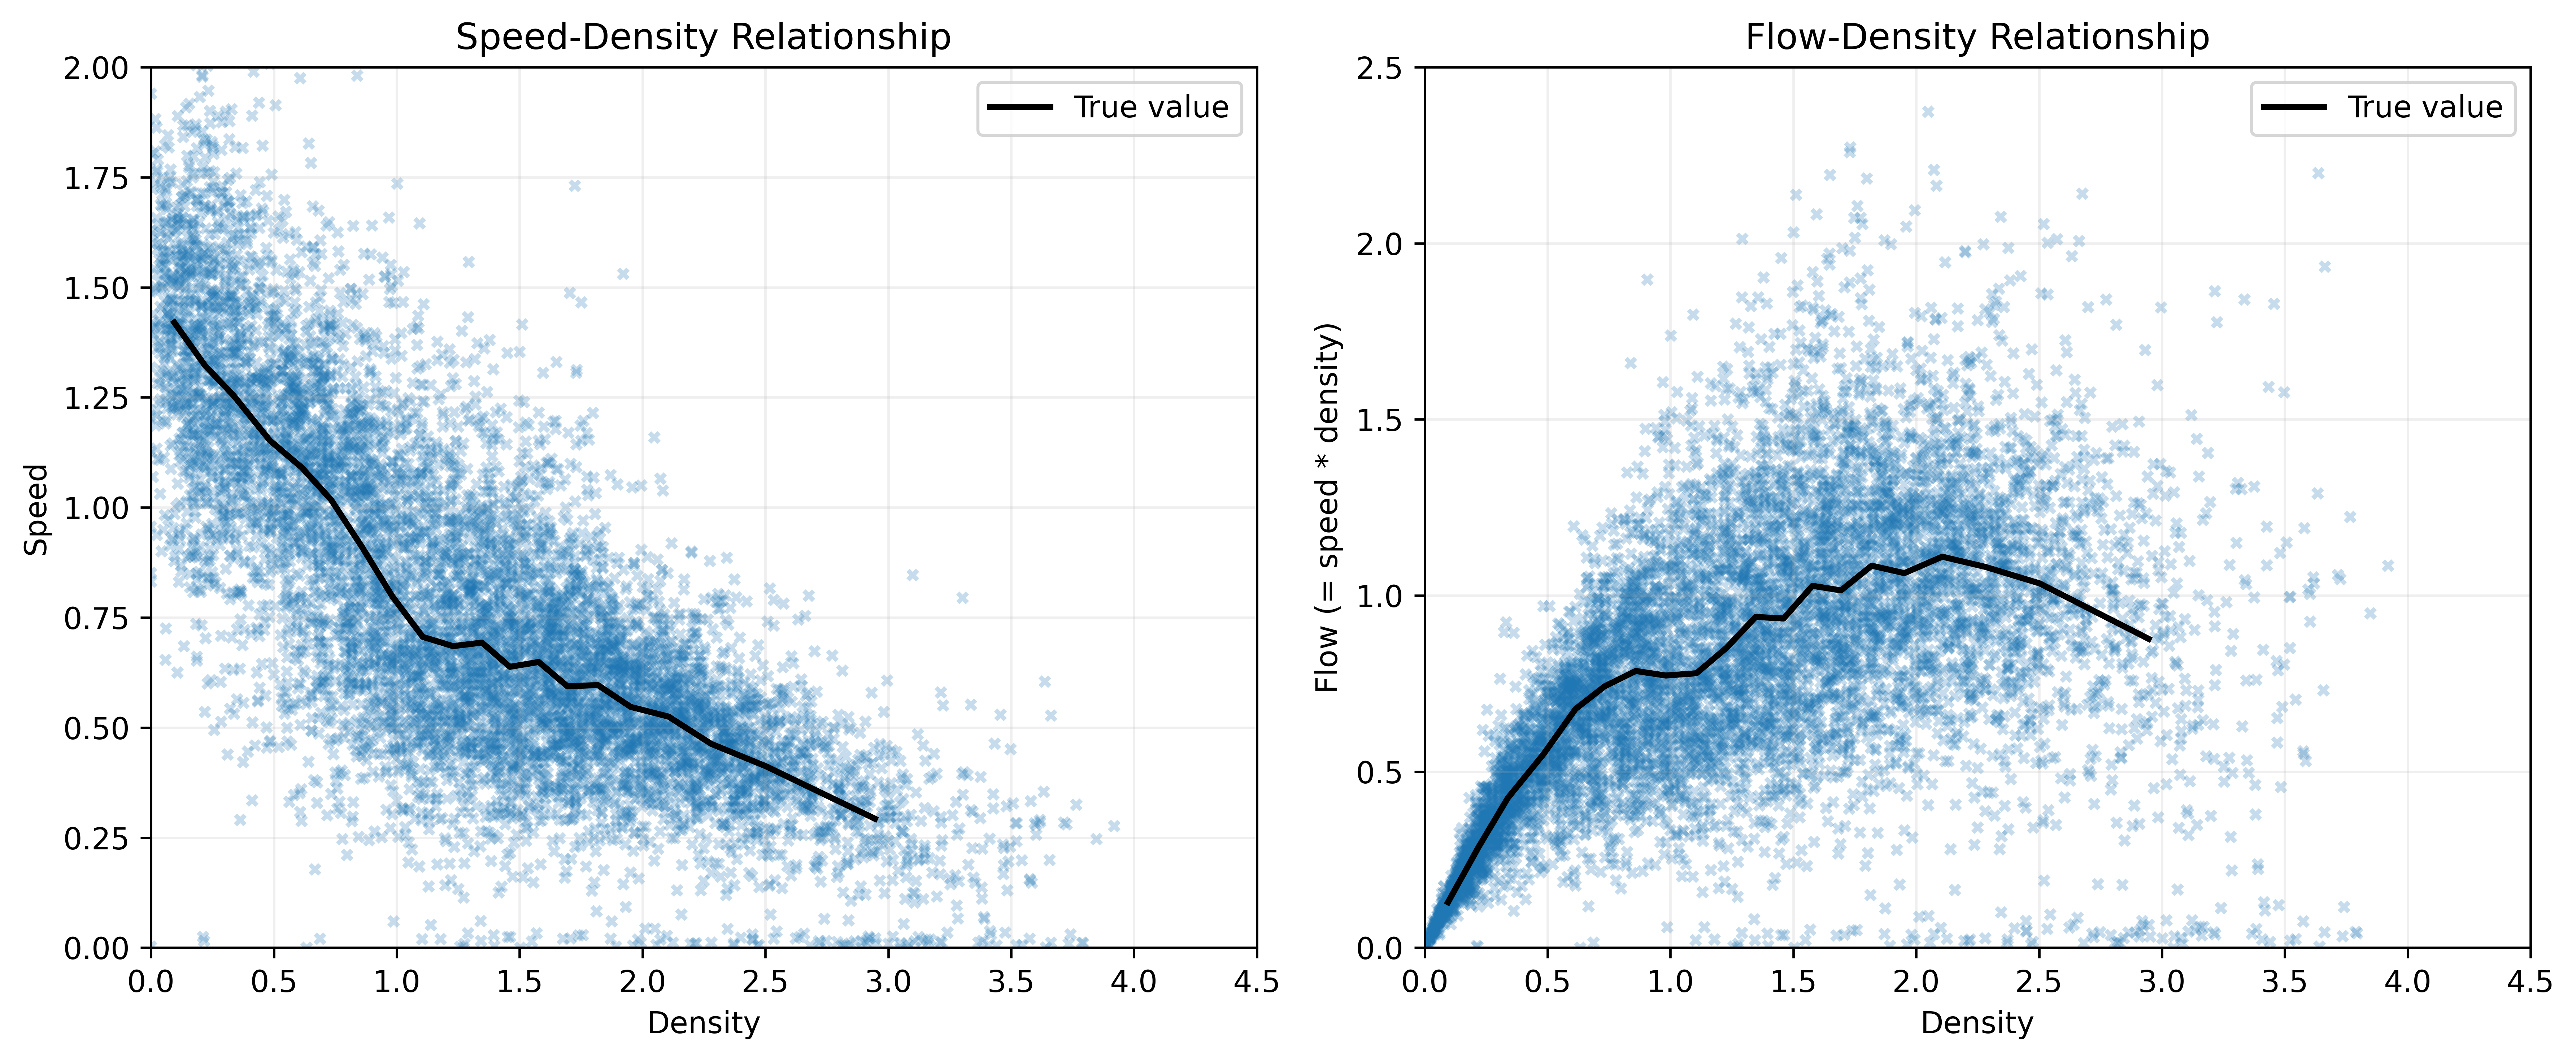
\includegraphics[width=1.0\linewidth]{fig/paradigm_obs.png}
    \caption{Empirical speed--density and flow--density relationships from controlled laboratory corridor experiments~\citep{zhangjun2013}.}
    \label{fig:fundamental_diagram_obs}
\end{figure}


Based on the empirical observations, we fit a generalized exponential (Underwood-type) fundamental diagram. The parameters are estimated via constrained nonlinear least squares:
\begin{equation}
(\hat v_f,\hat \rho_0,\hat n)=
\arg\min_{v_f>0,\ \rho_0>0,\ n>0}
\sum_{j=1}^{M}\Big(v_j- v_f\exp\!\big(-(\rho_j/\rho_0)^n\big)\Big)^2 .
\label{eq:nlls_calibration}
\end{equation}
The calibrated parameters are $\hat v_f=1.574~\mathrm{m/s}$, $\hat \rho_0=1.735~\mathrm{ped/m^2}$, and $\hat n=0.852$
with $\mathrm{RMSE}=0.037~\mathrm{m/s}$. The fitted curve is used as a macroscopic mobility constraint and further yields the
corresponding flow--density relation $q(\rho)=\rho v(\rho)$.


\subsection{Corridor-scale Validation and Quantitative Error Analysis}
\label{sec:validation_metrics}


We next run corridor simulations using the calibrated SPH-based movement model, and extract $(\rho, v)$ pairs from
trajectories to compute speed--density and flow--density relationships. Figure~\ref{fig:fundamental_diagram_sim} visualizes
the simulated fundamental diagrams, which closely follow the empirical trend across the tested density range.

\begin{figure}[htbp]
    \centering
    
\includegraphics[width=1.0\linewidth]{fig/paradigm_passage_sim.png}
    \caption{Simulated fundamental diagrams in corridor experiments using the calibrated SPH-based model.}
    \label{fig:fundamental_diagram_sim}
\end{figure}

To quantify the agreement between the simulated and empirical fundamental diagrams, we compute the Root Mean Square Error
(RMSE) and the coefficient of determination ($R^2$):
\begin{equation}
\mathrm{RMSE} = \sqrt{ \frac{1}{N} \sum_{i=1}^{N} \big(y_{\mathrm{sim}, i} - y_{\mathrm{obs}, i}\big)^2 },
\label{eq:rmse}
\end{equation}
\begin{equation}
R^2 = 1 - \frac{\sum_{i=1}^{N} \big(y_{\mathrm{sim}, i} - y_{\mathrm{obs}, i}\big)^2}
{\sum_{i=1}^{N} \big(y_{\mathrm{obs}, i} - \bar{y}_{\mathrm{obs}}\big)^2}.
\label{eq:r2}
\end{equation}

We compare the empirical baseline (Dataset~1) and the corridor simulation outputs (Dataset~2) using binned-median curves
evaluated on shared density bins ($N_{\mathrm{bins}}=24$ effective bins with sufficient samples).
For the \textbf{speed--density} relationship, the simulation achieves $\mathrm{RMSE}=0.085$ and $R^2=0.943$,
indicating excellent agreement in both magnitude and variation across densities. For the \textbf{flow--density} relationship,
the agreement remains strong with $\mathrm{RMSE}=0.110$ and $R^2=0.810$, while moderate deviations occur at high densities
where throughput becomes highly sensitive to local interactions and transient stop-and-go fluctuations.
\revb{These results indicate that the calibrated movement relationship reproduces the tested corridor-level
speed--density and flow--density trends. They provide component-level empirical support for the movement model, but do
not independently validate absolute settlement-scale clearance time, population allocation, exit choice, or detailed
spatial congestion. The protocol used to examine those case-scale outputs is outlined in
Section~\ref{sec:case_scale_protocol}, with the corresponding results reported in
Section~\ref{sec:macro_verification}.}

\subsection{Scope of Validation and Case-scale Verification Protocol}
\label{sec:case_scale_protocol}

\revb{Because controlled full-community evacuation observations and building-level occupancy data are generally
unavailable, settlement-scale outputs are evaluated through verification and plausibility checks rather than treated as
directly field-validated forecasts. The assessment uses a paired design in which the baseline and a representative
intervention share identical initial pedestrian coordinates across multiple random seeds. Temporal consistency is
examined using the $t_{50}$, $t_{80}$, and $t_{95}$ clearance times and normalized population-time; spatial response is
examined using cell-level evacuation-time differences and residual-population trajectories; and physical plausibility is
checked against an actual-path free-flow lower bound. Together, these diagnostics test stochastic robustness, internal
consistency, and the spatial concentration of intervention effects. Their application to the case-study configuration is
presented after the baseline and optimization results in Section~\ref{sec:macro_verification}.}


\section{Experiments: A Case Study of Shipai Village, Guangzhou}
\label{sec:experiments}

This section evaluates the proposed evacuation simulation and optimization framework using a real-world case study from
Shipai Village, one of the densest urban informal settlements in Guangzhou, China. The analysis proceeds through six
components: (i) study-area description and digital reconstruction, (ii) baseline evacuation simulation and risk analysis,
(iii) road-network optimization, (iv) village-scale macro verification and plausibility assessment, (v) sensitivity
analysis of the crowd model and optimization procedure, and (vi) computational-performance and empirical-scaling
assessment.

% =======================================================
\subsection{Computational Environment Construction and Preparation}
\label{sec:studyarea}

\begin{figure}[h]
\centering
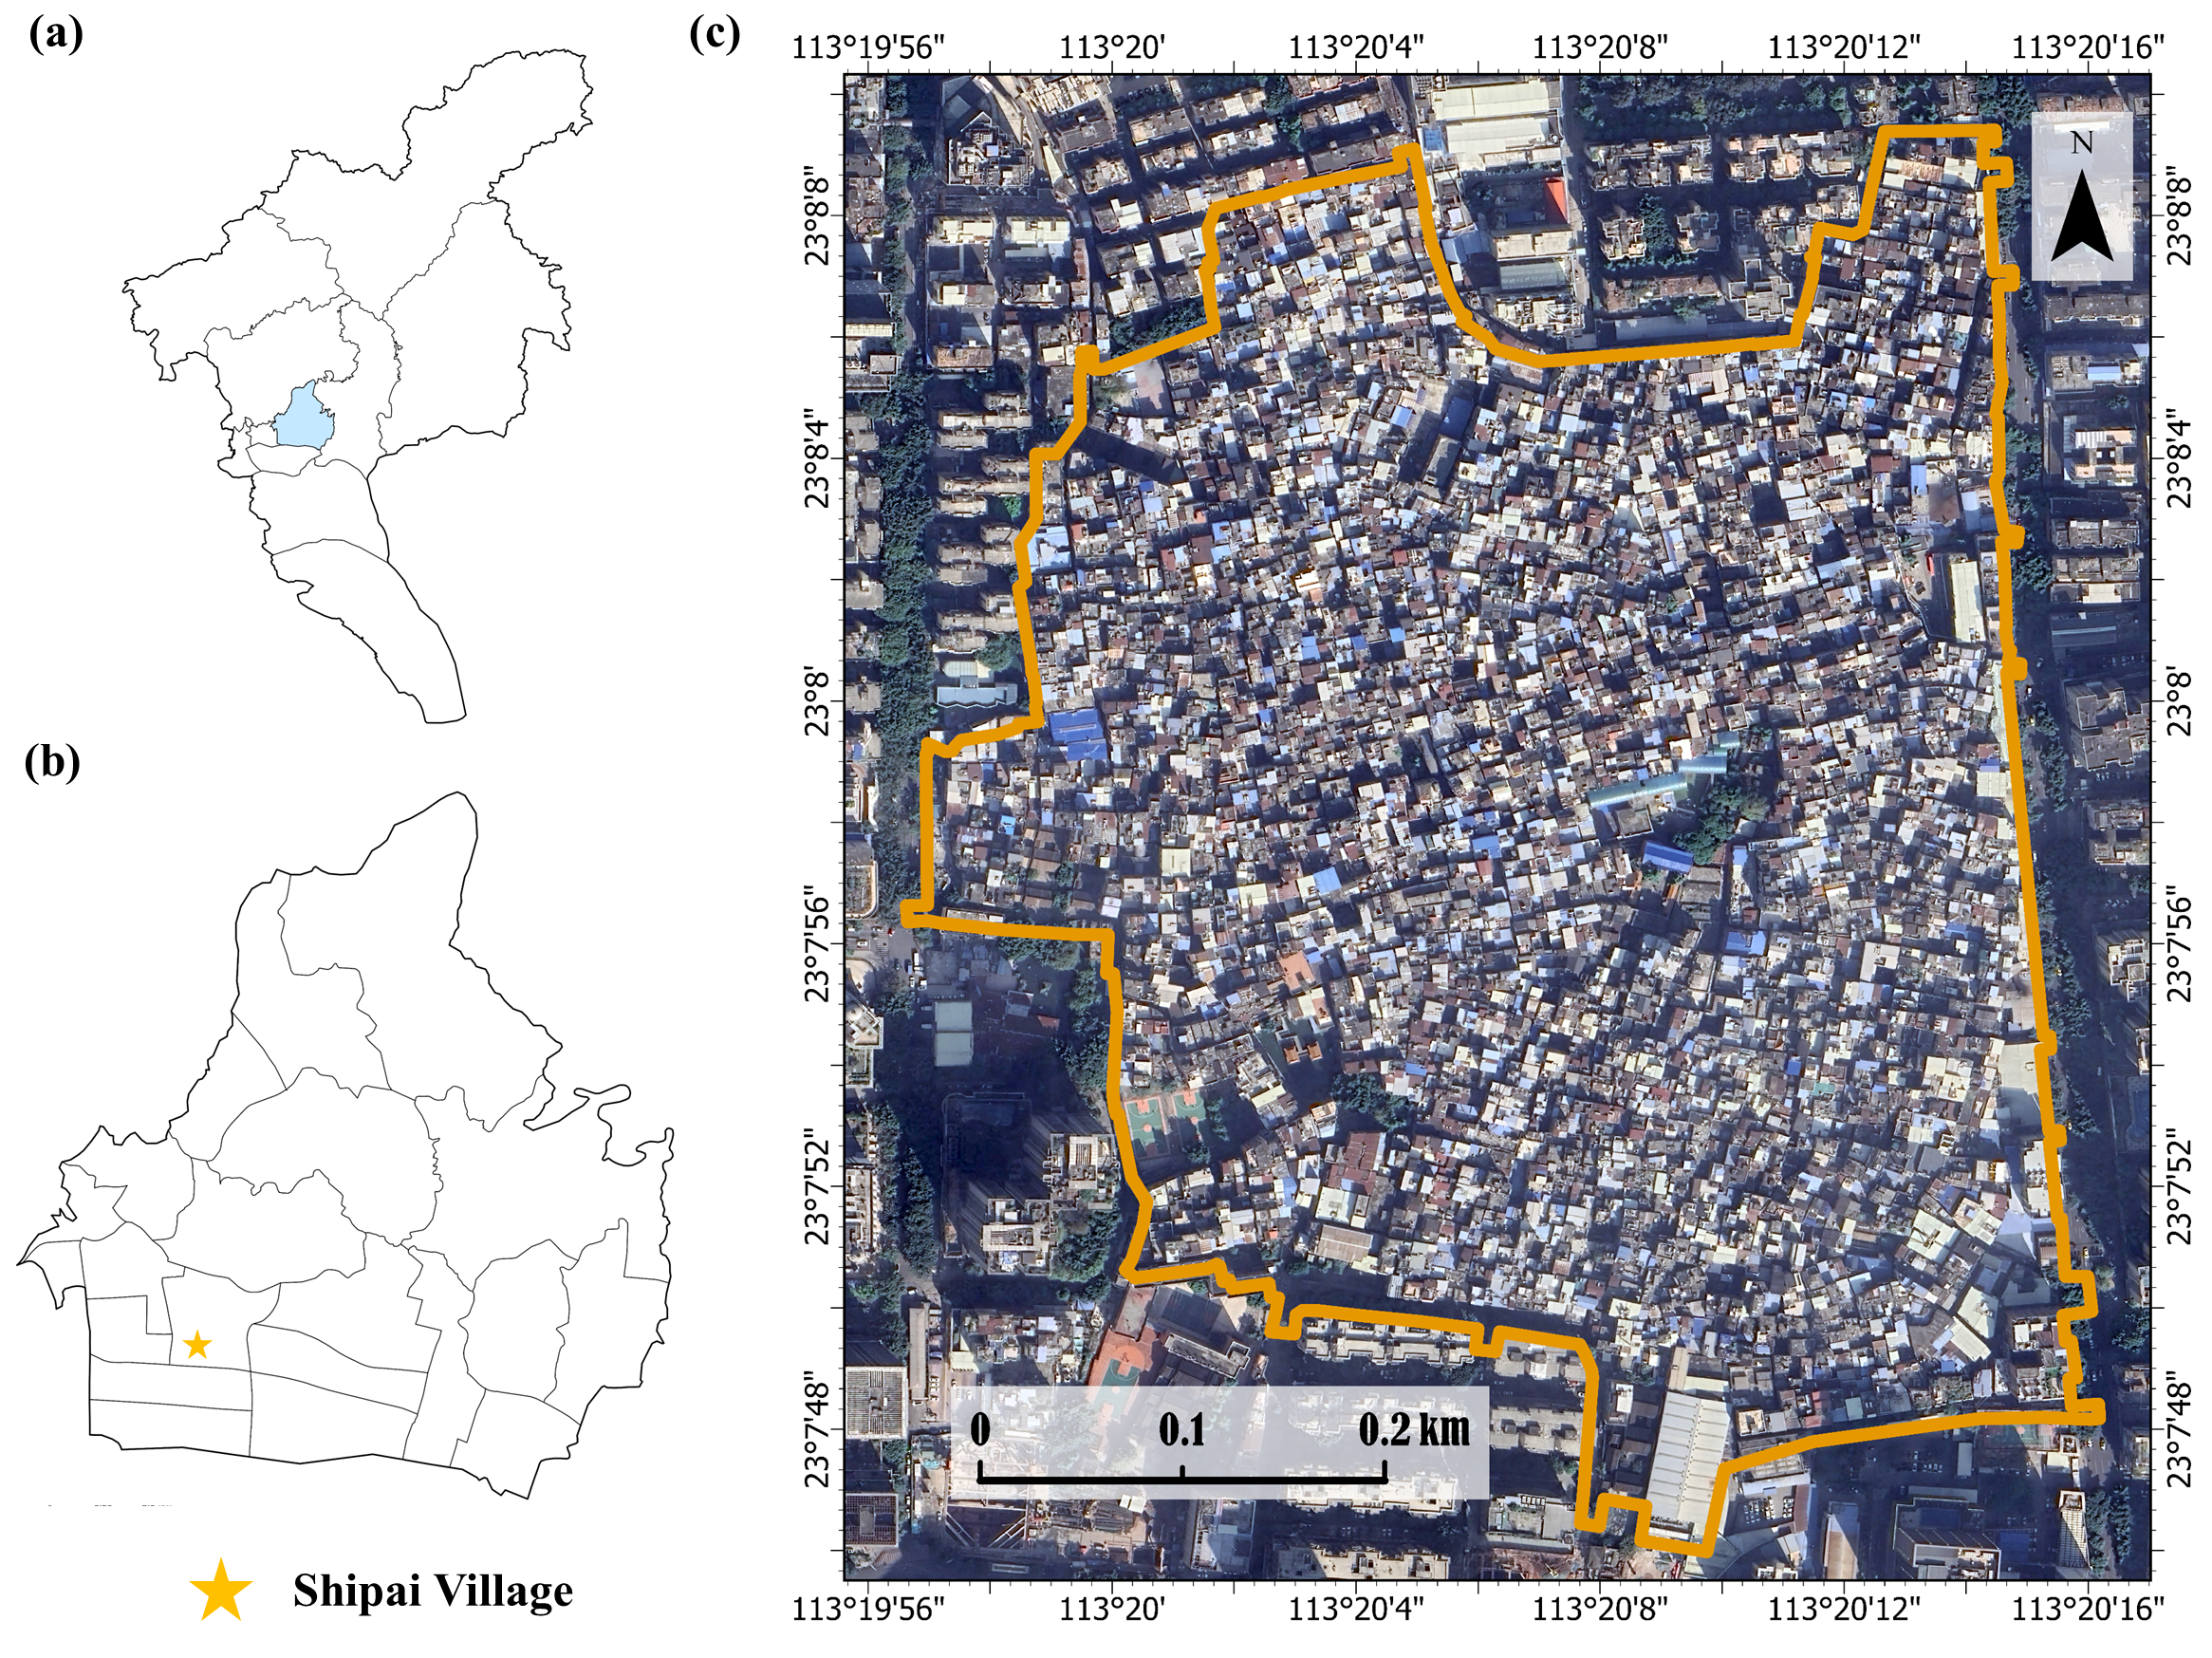
\includegraphics[width=1.0\linewidth]{fig/shipai_seli.png}
\caption{Map of study area. (a) Guangzhou, China.
(b) Zoomed-in view of Tianhe District in Guangzhou.
(c) Satellite remote-sensing image of Shipai Village, the orange boundary highlights the administrative extent.}
% \caption{Panels (a), (b), and (c) show the geographic locations of Guangdong Province, Guangzhou City, and Shipai Village, respectively.  The yellow outline in Panel (c) indicates the administrative boundary of the village.}
\label{fig:study_area}
\end{figure}


Shipai Village is a high-density urban settlement located in Tianhe District, Guangzhou, China, as illustrated in Figure~\ref{fig:study_area}. The computational study area covers approximately 80\,ha. A public report describes the village as containing approximately 3500 tightly packed buildings and a historical population approaching 100,000\footnote{\textit{Guangzhou Daily}: \url{https://news.sina.cn/2014-12-11/detail-icczmvun1836822.d.html}}. Because many adjoining houses share walls and cannot be reliably delineated as separate footprints, spatially contiguous structures were merged during preprocessing, yielding 1660 building aggregates used as the computational units in this study. The internal circulation system is dominated by narrow corridors and alleys, with typical widths of 0.8--3\,m and only a few small open spaces or squares; field reporting likewise notes that the main roads are generally only 2--3\,m wide and inaccessible to large vehicles\footnote{\textit{Yangcheng Evening News}: \url{https://ycpai.ycwb.com/ycppad/content/2020-01/09/content_613007.html}}. Although the population has declined in recent years, its current size remains uncertain. We therefore adopt 50,000 evacuees as a deliberately demanding stress-test scenario rather than as a definitive estimate of the present population.

High-resolution building footprints were obtained from remote sensing imagery and cadastral data, and were manually cleaned to correct misalignments and remove non-residential structures. Based on this, the computational domain was defined and discretized into a regular grid with a spatial resolution of 0.1\,m, which is sufficient to capture the fine-scale geometry of the corridors and small intersections.




\begin{figure}
\centering
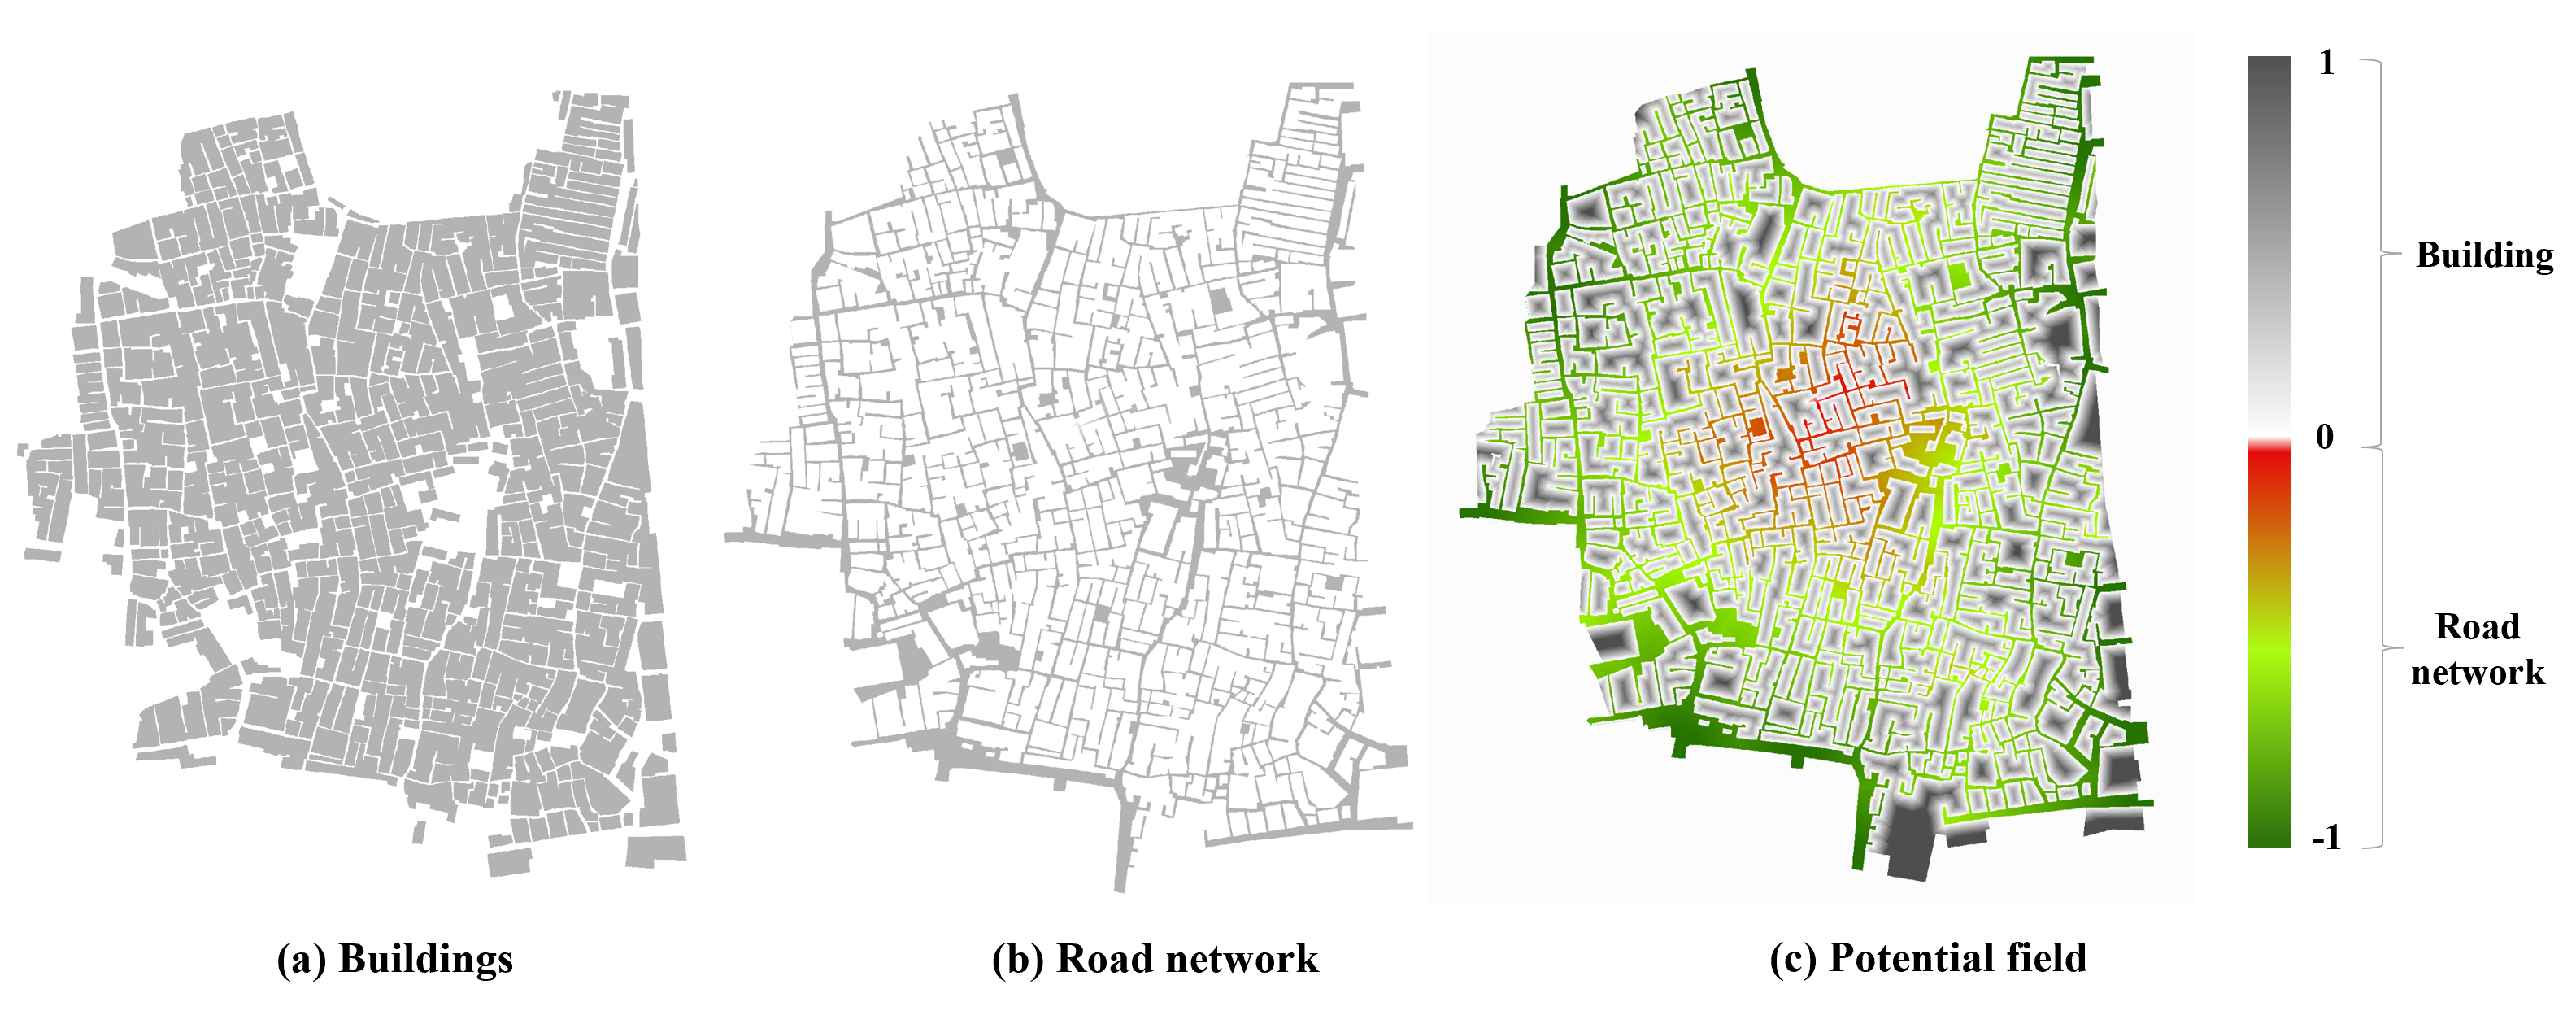
\includegraphics[width=1\linewidth]{fig/Snipaste_2025-12-11_19-43-55.png}
\caption{Road network layout of Shipai Village and the derived navigation potential field.
(a) Buildings; (b) Road network; (c) Navigation potential field.}
\label{fig:shipai_navigation}
\end{figure}

Figure~\ref{fig:shipai_navigation} summarizes the rasterized environment and the derived global navigation field for Shipai Village. Walkable space is obtained by subtracting building footprints from the study area and rasterizing the remaining free-space region. Given 16 boundary exits selected from planning documents and field observations, we compute a multi-source Dijkstra distance potential $\Phi(\mathbf{x})$ on the weighted walkable grid with buildings treated as impassable obstacles. The negative gradient $-\nabla \Phi$ provides a globally consistent navigation field that steers pedestrians to the nearest feasible exit. In the visualization, warmer colors indicate larger distance-to-exit potential, and streamlines highlight dominant evacuation routes converging to the exits.


% =======================================================
\subsection{Baseline Evacuation Simulation and Risk Analysis}
\label{sec:baseline}

This section serves two purposes. First, it establishes the \emph{baseline} evacuation performance under the original
road layout, which will be used as the reference for evaluating the post-renovation improvements in
Section~\ref{sec:exp_setup}. Second, it performs a simulation-based \emph{risk diagnosis} to identify persistent
congestion hotspots and high-risk links, which subsequently define the candidate set for targeted road widening.

\revb{A total of $N=50{,}000$ pedestrians were generated under the study's floor-area-based allocation rule, with uniform occupancy assumed within each building. This population was deliberately adopted as a demanding stress-test scenario, reflecting the settlement's historically large tenant population while recognizing its population decline in recent years; it should therefore not be interpreted as a precise estimate of the current population. The detailed allocation is also a scenario assumption because building-level occupancy observations are unavailable. The simulation time step was $\Delta t=0.1$~s, the maximum walking speed was 1.6~m/s, and the implemented baseline neighborhood length was $h=2.4$~m. Pedestrians follow the global navigation field while adjusting their movement through local interaction and density-dependent speed regulation.}

\begin{figure}[htbp]
\centering

\includegraphics[width=1\linewidth]{fig/hist_time_distance.png}
\caption{Baseline evacuation outcomes under the original layout:
histograms of evacuation time (left) and travel distance (right).}
\label{fig:evacuation_time_distance}
\end{figure}

% \paragraph{Baseline evacuation performance.}
Figure~\ref{fig:evacuation_time_distance} reports the distributions of individual evacuation travel distance and evacuation
time for agents who successfully reached an exit. In terms of travel distance, \textbf{93.77\%} of evacuees complete their
trips within \textbf{300 m}, indicating that most origins are relatively close to available exits, whereas a small tail of
longer routes remains. Regarding evacuation time, \textbf{87.73\%} of evacuees finish within \textbf{400 s}, suggesting that
the majority can evacuate within a moderate time window, but a subset experiences prolonged delays due to detours and
queueing in narrow, poorly connected alleys. Overall, both metrics exhibit a right-skewed pattern: the bulk population
evacuates efficiently, whereas the long-tail evacuees---often originating from interior dead-ends or bottleneck-prone
corridors---dominate the final clearance stage and constitute the most critical cases for micro-regeneration.

\begin{figure}[htbp]
\centering
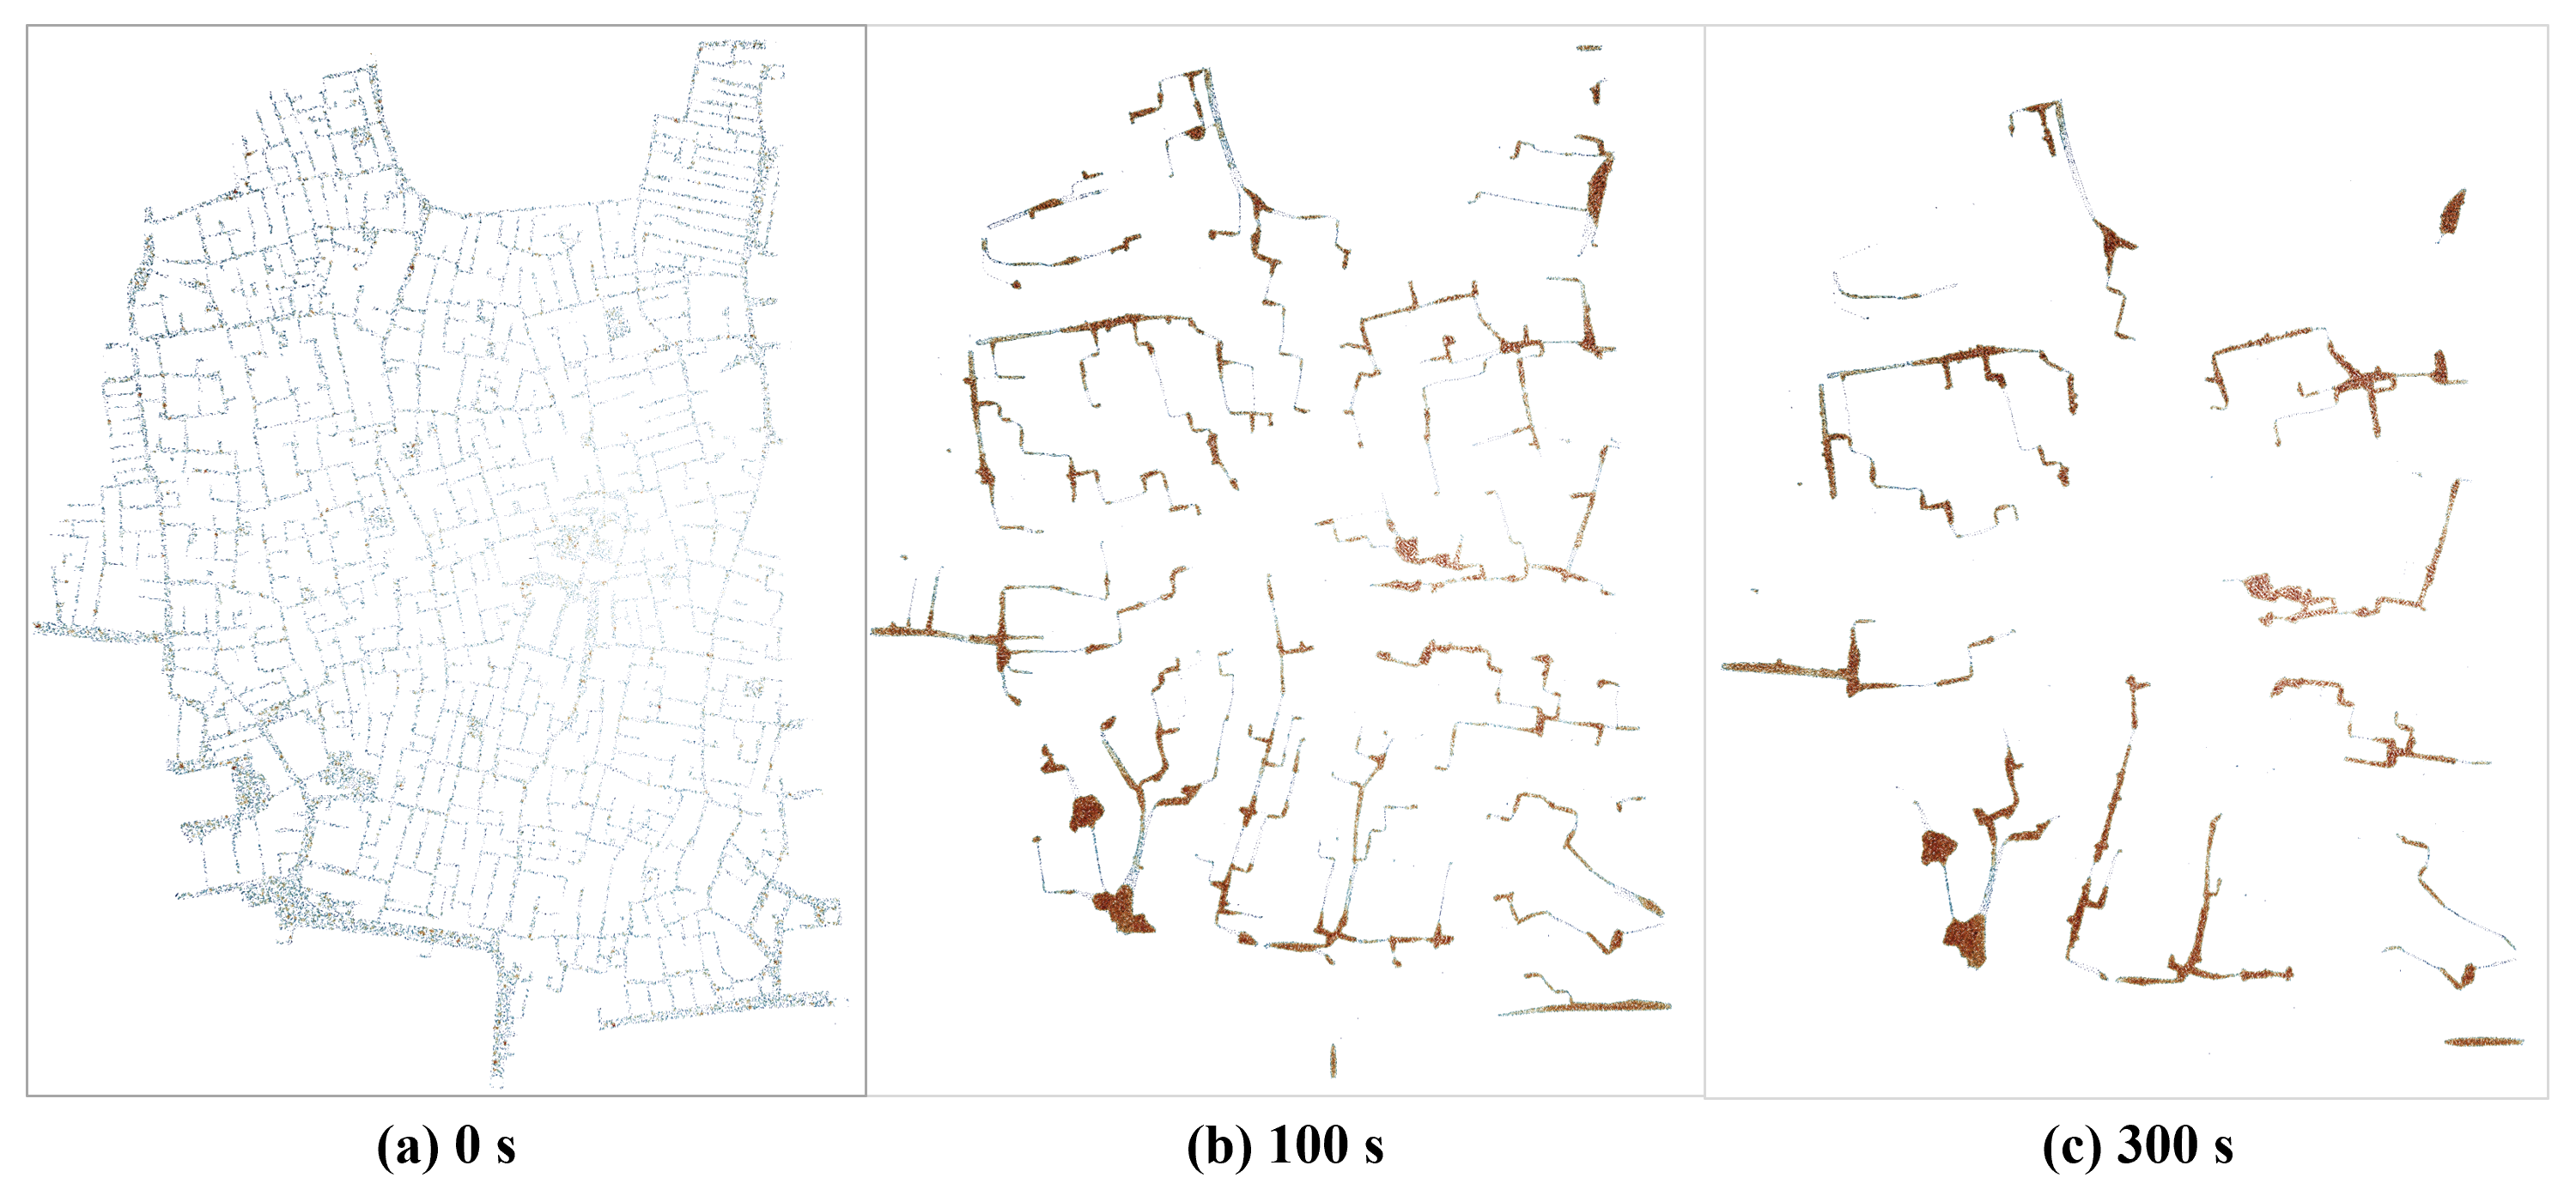
\includegraphics[width=0.8\linewidth]{fig/simulation_process_1.png}\\
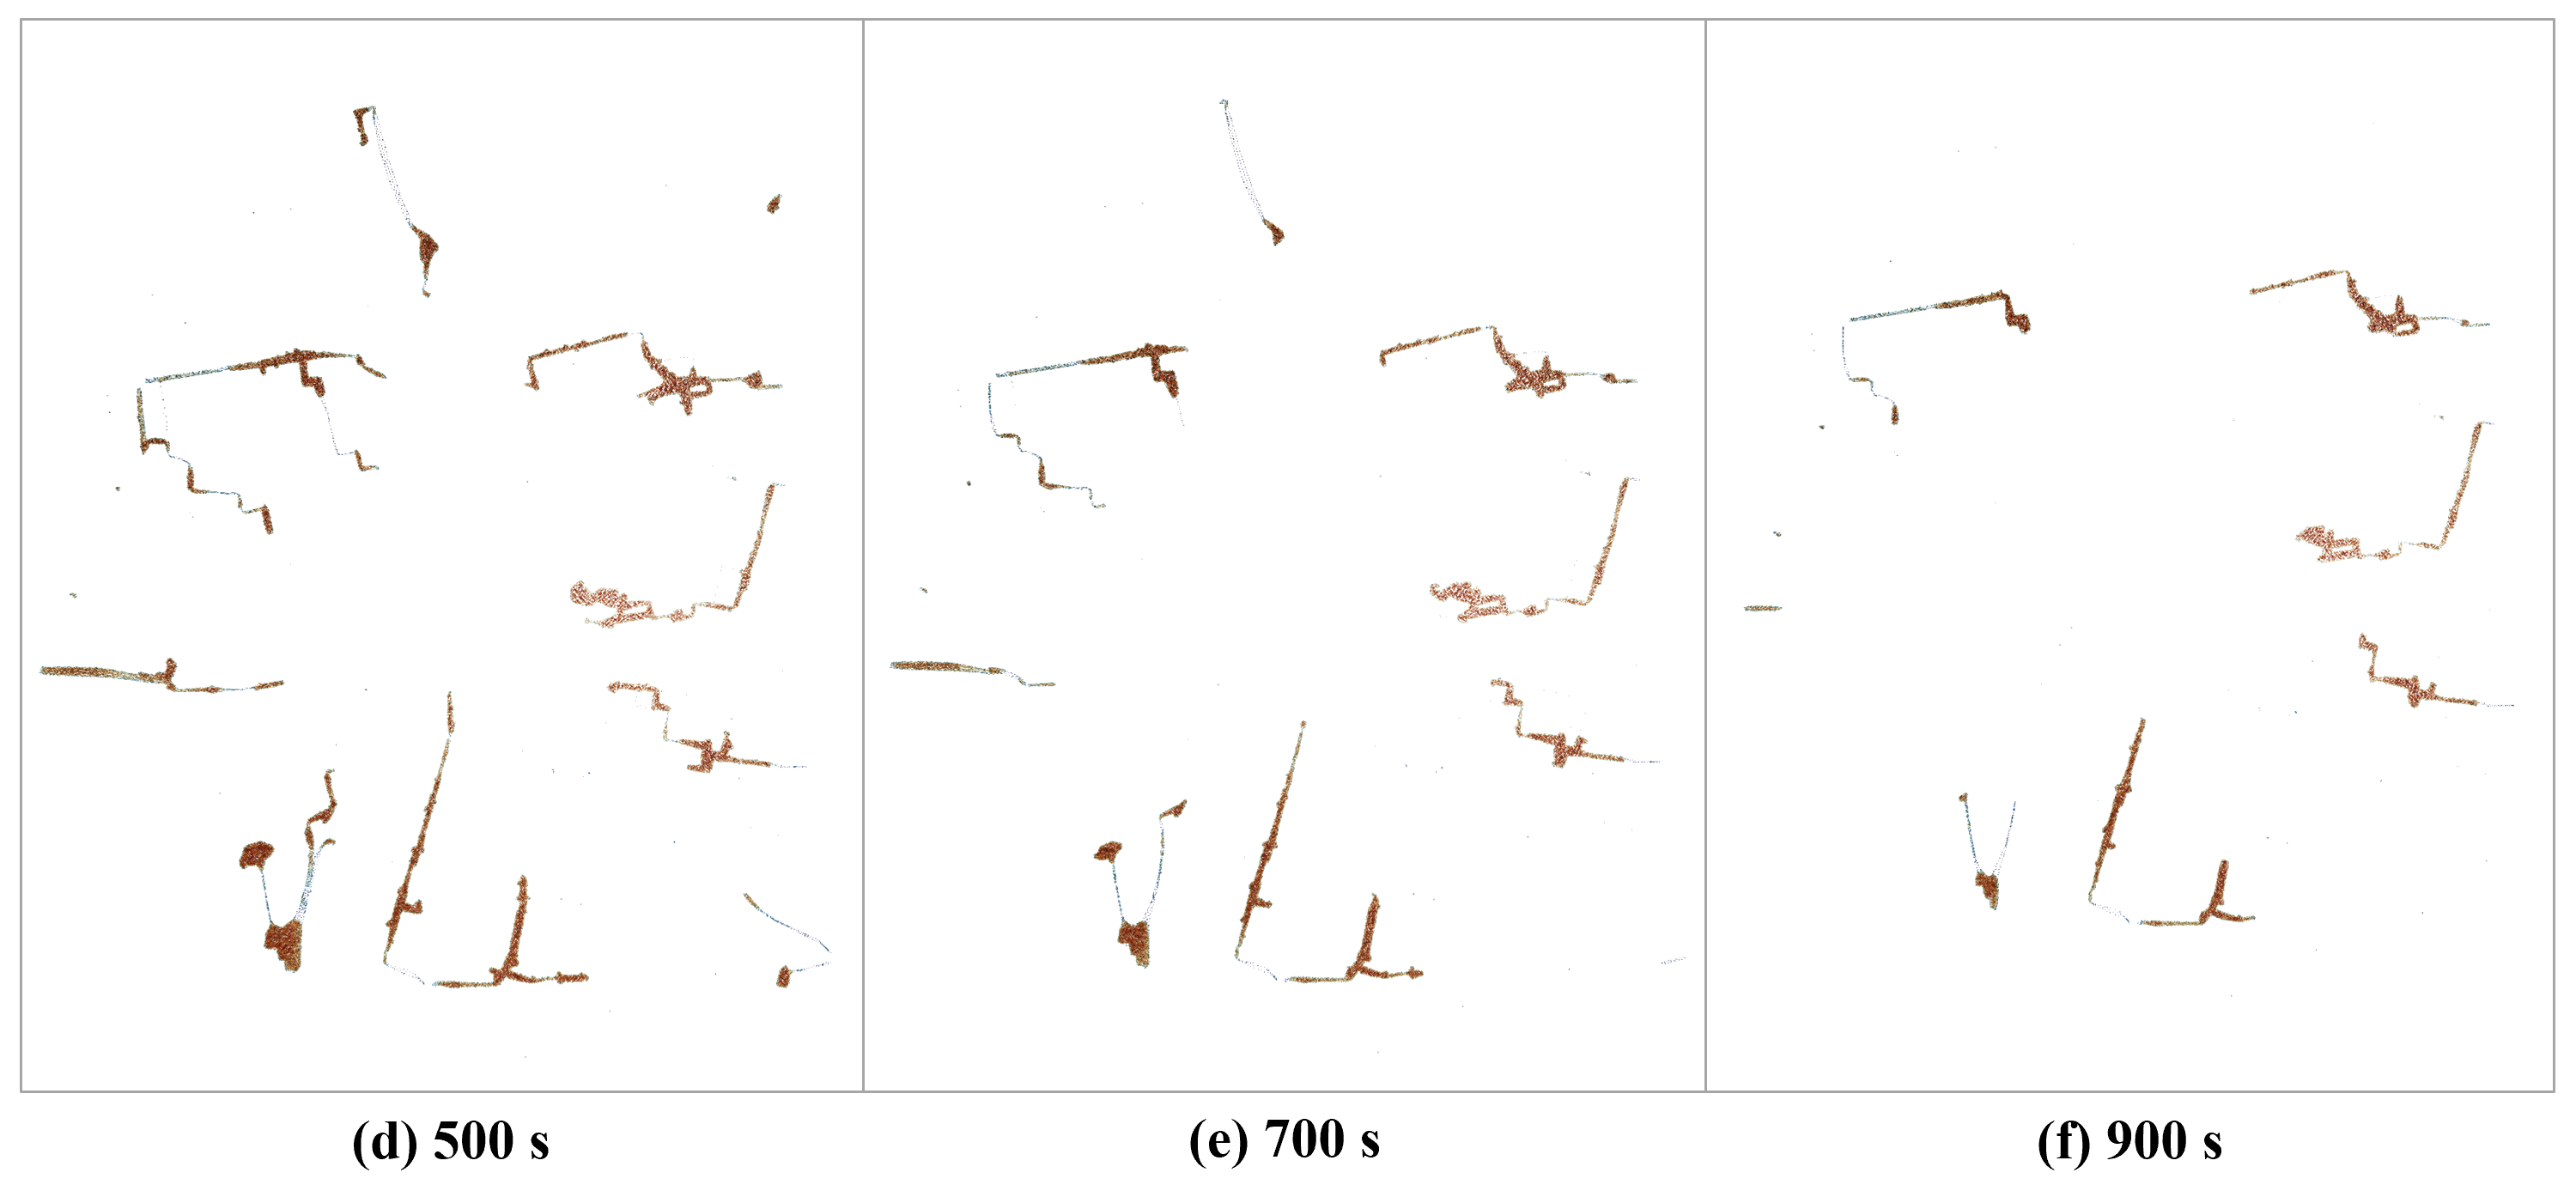
\includegraphics[width=0.8\linewidth]{fig/simulation_process_2.png}
\caption{Snapshots of the evacuation process under the original layout at $0$, $100$, $300$, $500$, $700$, and $900$~s.}
\label{fig:simulation_layout}
\end{figure}


To illustrate the dynamic evolution, Figure~\ref{fig:simulation_layout} shows snapshots of the evacuation process at
$0$, $100$, $300$, $500$, $700$, and $900$~s. The results reveal total process congestion accumulation along the main corridor and
at junctions where multiple narrow alleys merge, followed by a prolonged clearance phase dominated by interior residents
from deep cul-de-sacs.


% \paragraph{\textbf{Spatio-temporal congestion and risk mapping}}
Following the Phase~I procedure described in Section~\ref{sec:method_bottleneck}, we evaluate the baseline layout using
the two cumulative raster indicators defined in Eqs.~\eqref{eq:tcong} and~\eqref{eq:rhocong}: Cumulative Congestion Time
$T_{\mathrm{cong}}(\mathbf{p})$ and Cumulative Crowd Density $D_{\mathrm{cum}}(\mathbf{p})$.
Figure~\ref{fig:congestion_area} presents their spatial distributions under the original layout. High-value regions
concentrate along the primary corridors and at several junctions where multiple narrow alleys merge, showing where
low-speed pedestrian exposure and crowd-density exposure repeatedly accumulate during the evacuation.



\begin{figure}[htbp]
\centering

\includegraphics[width=1\linewidth]{fig/cumulative_time_density.png}
\caption{Spatial distribution of cumulative congestion metrics under the original layout of Shipai Village:
(a) Cumulative Congestion Time, $T_{\mathrm{cong}}(\mathbf{p})$, and (b) Cumulative Crowd Density,
$D_{\mathrm{cum}}(\mathbf{p})$. Warmer colors indicate greater cumulative exposure; exits are marked as \emph{Exit}.}
\label{fig:congestion_area}
\end{figure}


\begin{figure}[htbp]
    \centering
    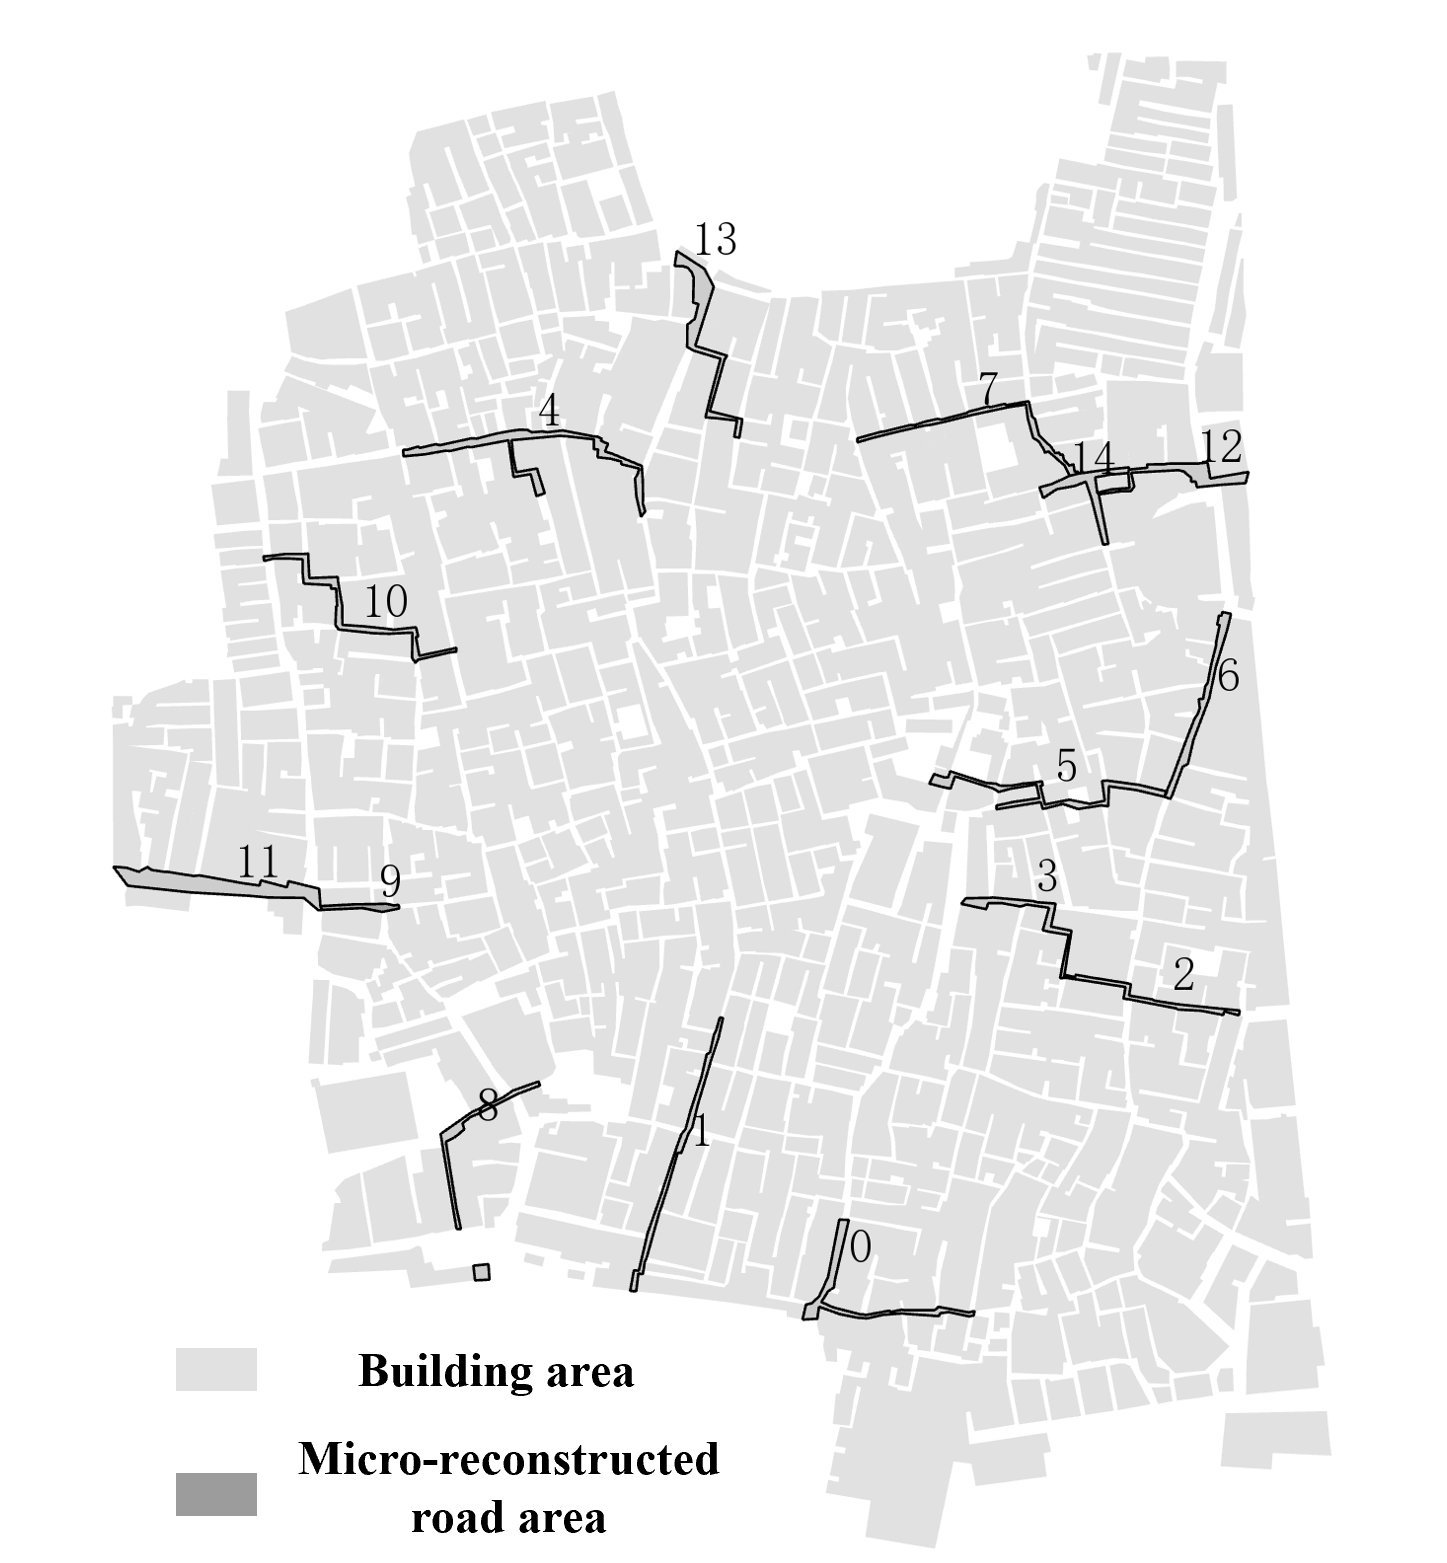
\includegraphics[width=0.5\linewidth]{fig/micro_reconstructed_area.png}
    \caption{Spatial distribution of road segments identified as high-risk candidates for reconstruction based on simulation results.}
    \label{fig:micro_reconstruction}
\end{figure}


The candidate bottleneck road segments obtained through the clustering and network-mapping procedure described in
Section~\ref{sec:method_bottleneck} are shown in Figure~\ref{fig:micro_reconstruction}. These segments are retained as
the intervention candidate set for the discrete widening optimization in Section~\ref{sec:exp_setup}.


% =========================================================
% Experiments (matched to the Method section)
% Place this under: \section{Experiments and Results}
% =========================================================
% Superseded single-objective result block retained in source for provenance only.
\iffalse
\subsection{Road Network Optimization}
\label{sec:exp_setup}

To validate the proposed targeted micro-regeneration framework,
we conduct a simulation-driven optimization experiment on the Shipai Village scenario.
All candidate interventions are evaluated using a C$++$-based evacuation simulator, which outputs
(i) the remaining-evacuee time series for computing $F_{\mathrm{evac}}$,
and (ii) raster-level metadata (e.g., affected building-cell counts) for estimating the demolition/land-take proxy $F_{\mathrm{cost}}$.




A baseline SPH evacuation simulation is first executed on the original raster map to detect critical congestion zones. These zones are mapped to a set of candidate bottleneck segments, yielding
$K$ discrete decision variables. During optimization, each candidate vector
$\boldsymbol{x}=[\delta_1,\dots,\delta_K]\in\mathcal{D}^K$ updates the local road widths, after which the simulator is
executed to obtain evacuation dynamics and metadata required to estimate reconstruction cost.



For each solution $\boldsymbol{x}$ generated by the GA, we: (1) update simulator inputs (project name,
road-width configuration, and crowd settings), (2) run the C++ simulator, (3) compute the evacuation score
$F_{\mathrm{evac}}(\boldsymbol{x})$, and (4) compute the raster-based intervention-cost proxy
$F_{\mathrm{cost}}(\boldsymbol{x})$ from raster metadata. All evaluated solutions and their objective values are logged
to a CSV file for reproducibility and post-analysis.
The parameter settings are detailed in Table \ref{tab:exp_params}.



\begin{table}[htbp]
\centering
\caption{Experimental parameter settings.}
\label{tab:exp_params}
\begin{tabular}{l c}
\hline
\textbf{Category} & \textbf{Value} \\
\hline
\multicolumn{2}{l}{\textit{Scenario and simulation}} \\
\hline
Project / scenario ID & \texttt{shipai\_0} (baseline) \\
Crowd size & 50{,}000 agents \\
Raster resolution & $0.1$ m \\
Simulator & C++ executable (\texttt{./1213}) \\
\hline
\multicolumn{2}{l}{\textit{Decision variables}} \\
\hline
Number of bottleneck segments & $K{=}15$ \\
Widening set & $\mathcal{D}=\{0,2,4\}$ m \\
\hline
\multicolumn{2}{l}{\textit{Objective function}} \\
\hline
Evacuation weight & $\alpha = 1.0$ \\
Illustrative post-hoc preference & $\beta = 0.1$ (not used to construct the front) \\
Reconstruction-cost coefficient & $c = 1.0$ (relative unit/m$^{2}$) \\
\hline
\multicolumn{2}{l}{\textit{Evolutionary algorithm}} \\
\hline
Population size & 40 \\
Offspring batches & 25 \\
Selection strategy & Rank--crowding binary tournament \\
Crossover operator (prob.) & Uniform crossover ($p_c=0.8$) \\
Mutation operator (prob.) & Gene-wise discrete replacement ($p_m=0.08$) \\
Environmental selection & $(\mu+\lambda)$ NSGA-II selection \\
Simulator calls per optimizer seed & $40+25\times40=1040$ \\
Optimizer seeds & 11, 29, and 47 \\
Total simulator calls & $3120$ \\
\hline
\end{tabular}
\end{table}

\begin{figure}[htbp]
\centering

\includegraphics[width=1\linewidth]{fig/ga_7_1.png}
\caption{Convergence behavior and objective trade-off of the genetic algorithm across generations.}
\label{fig:conv_curve}
\end{figure}

% \subsubsection{Optimization results and analysis}
Figure~\ref{fig:conv_curve} shows the evolution of the best and average fitness values across generations, together with
the empirical cost--performance distribution of evaluated solutions. The best fitness decreases steadily and stabilizes
in later generations, indicating stable convergence of the simulation-in-the-loop search under the chosen operators and
hyperparameters.


\
\
Compared with the baseline (no widening) scenario, the selected optimized solution $\boldsymbol{x}_{\mathrm{opt}}$ achieves:
\begin{itemize}
    \item a reduction in total evacuation time $T$ by \textbf{143 s (14.3\%)},
    \item a reduction in evacuation score $F_{\mathrm{evac}}$ by \textbf{9.48\%},
    \item a raster-based demolition/land-take proxy $F_{\mathrm{cost}}$ of \textbf{347.46}
          relative units, corresponding to the affected building area represented by the raster metadata.
\end{itemize}


The best solution returned by the GA is
\[
\boldsymbol{x}_{\mathrm{opt}}=[0,0,2,0,0,0,0,0,0,2,0,0,4,0,0],
\]
which concentrates interventions on three segments: roads \#3, \#10, and \#13 are widened by $2$~m, $2$~m, and $4$~m,
respectively, while all other candidate segments remain unchanged. This highly sparse pattern suggests that, under the
given cost--performance trade-off, prioritizing a small number of critical bottlenecks is more effective than distributing
small upgrades across many locations.

\begin{figure}[htbp]
\centering

\includegraphics[width=1.0\linewidth]{fig/Fig4_road_widening_frequency_2m_4m.png}
\caption{Widening preference of road segments: selection frequency of 2~m and 4~m widening across evaluated solutions. Road indices correspond to those in Figure \ref{fig:micro_reconstruction}.}
\label{fig:widen_hist}
\end{figure}

To interpret the search preferences, we report the segment-wise selection frequencies across evaluated solutions
(Figure~\ref{fig:widen_hist}). In the \emph{2~m widening} group, road segments \#1, \#3, \#5, \#10, \#12, and \#14 exhibit the
highest occurrence frequencies, indicating that moderate widening on these roads tends to yield consistent evacuation
benefits with acceptable cost. In contrast, for the \emph{4~m widening} option, segment \#13 dominates with an occurrence
frequency close to $0.7$, while most other segments remain at low frequency (except segment \#3). This pattern implies that
aggressive widening (4~m) is cost-effective only for a very limited subset of bottlenecks (especially road \#13), whereas
for most segments the marginal evacuation gain is insufficient to justify the substantially higher demolition/land-take proxy.
Therefore, the derived optimum---$\{(\#3,2~\mathrm{m}),(\#10,2~\mathrm{m}),(\#13,4~\mathrm{m})\}$---is consistent with the
frequency evidence and supports the conclusion that selective, targeted widening is the most efficient micro-regeneration
strategy in this case.


\begin{figure}[htbp]
\centering

\includegraphics[width=1\linewidth]{fig/ga_7_2.png}
\caption{Diversity dynamics of the genetic algorithm across generations.
Left: population diversity (gene-wise standard deviation); right: discrete gene diversity measured by entropy.}
\label{fig:ga_diversity}
\end{figure}

Figure~\ref{fig:ga_diversity} reports the diversity dynamics of the GA.
Both population diversity (gene-wise standard deviation) and discrete gene entropy decrease over generations, indicating
a gradual concentration of the population toward a small subset of high-quality discrete widening patterns. This behavior
suggests that the evolutionary search converges rather than randomly drifting, and that the final solution is supported by
consistent selection preferences across the population (i.e., most segments tend to converge to $\delta=0$, while only a few
critical bottlenecks retain non-zero widening).




Overall, the simulation-driven optimization demonstrates that the proposed targeted micro-regeneration framework can
(i) identify a small set of high-impact bottlenecks from baseline congestion patterns, and (ii) allocate limited widening
budgets to achieve substantial evacuation improvement. The resulting intervention is sparse but effective, highlighting the
strong spatial heterogeneity of marginal widening benefits in dense and irregular urban-village road networks.
\fi

\subsection{Road Network Optimization}
\label{sec:exp_setup_revised}
\label{sec:exp_setup}

To validate the proposed targeted micro-regeneration framework,
we conduct a simulation-driven optimization experiment on the Shipai Village scenario.
All candidate interventions are evaluated using a C$++$-based evacuation simulator, which outputs
(i) the remaining-evacuee time series for computing $F_{\mathrm{evac}}$,
and (ii) raster-level metadata (e.g., affected building-cell counts) for estimating the demolition/land-take proxy $F_{\mathrm{cost}}$.

A baseline SPH evacuation simulation is first executed on the original raster map to detect critical congestion zones. These zones are mapped to a set of candidate bottleneck segments, yielding
$K$ discrete decision variables. During optimization, each candidate vector
$\boldsymbol{x}=[\delta_1,\dots,\delta_K]\in\mathcal{D}^K$ updates the local road widths, after which the simulator is
executed to obtain evacuation dynamics and cost-related metadata.

For each solution $\boldsymbol{x}$ generated by \revb{NSGA-II}, we: (1) update simulator inputs (project name,
road-width configuration, and crowd settings), (2) run the C++ simulator, (3) compute the evacuation score
$F_{\mathrm{evac}}(\boldsymbol{x})$, and (4) compute the raster-based intervention-cost proxy
$F_{\mathrm{cost}}(\boldsymbol{x})$ from raster metadata. All evaluated solutions and their objective values are logged
to a CSV file for reproducibility and post-analysis.
The parameter settings are detailed in Table~\ref{tab:exp_params_revised}.

\begin{figure}[htbp]
\centering
\revfloat
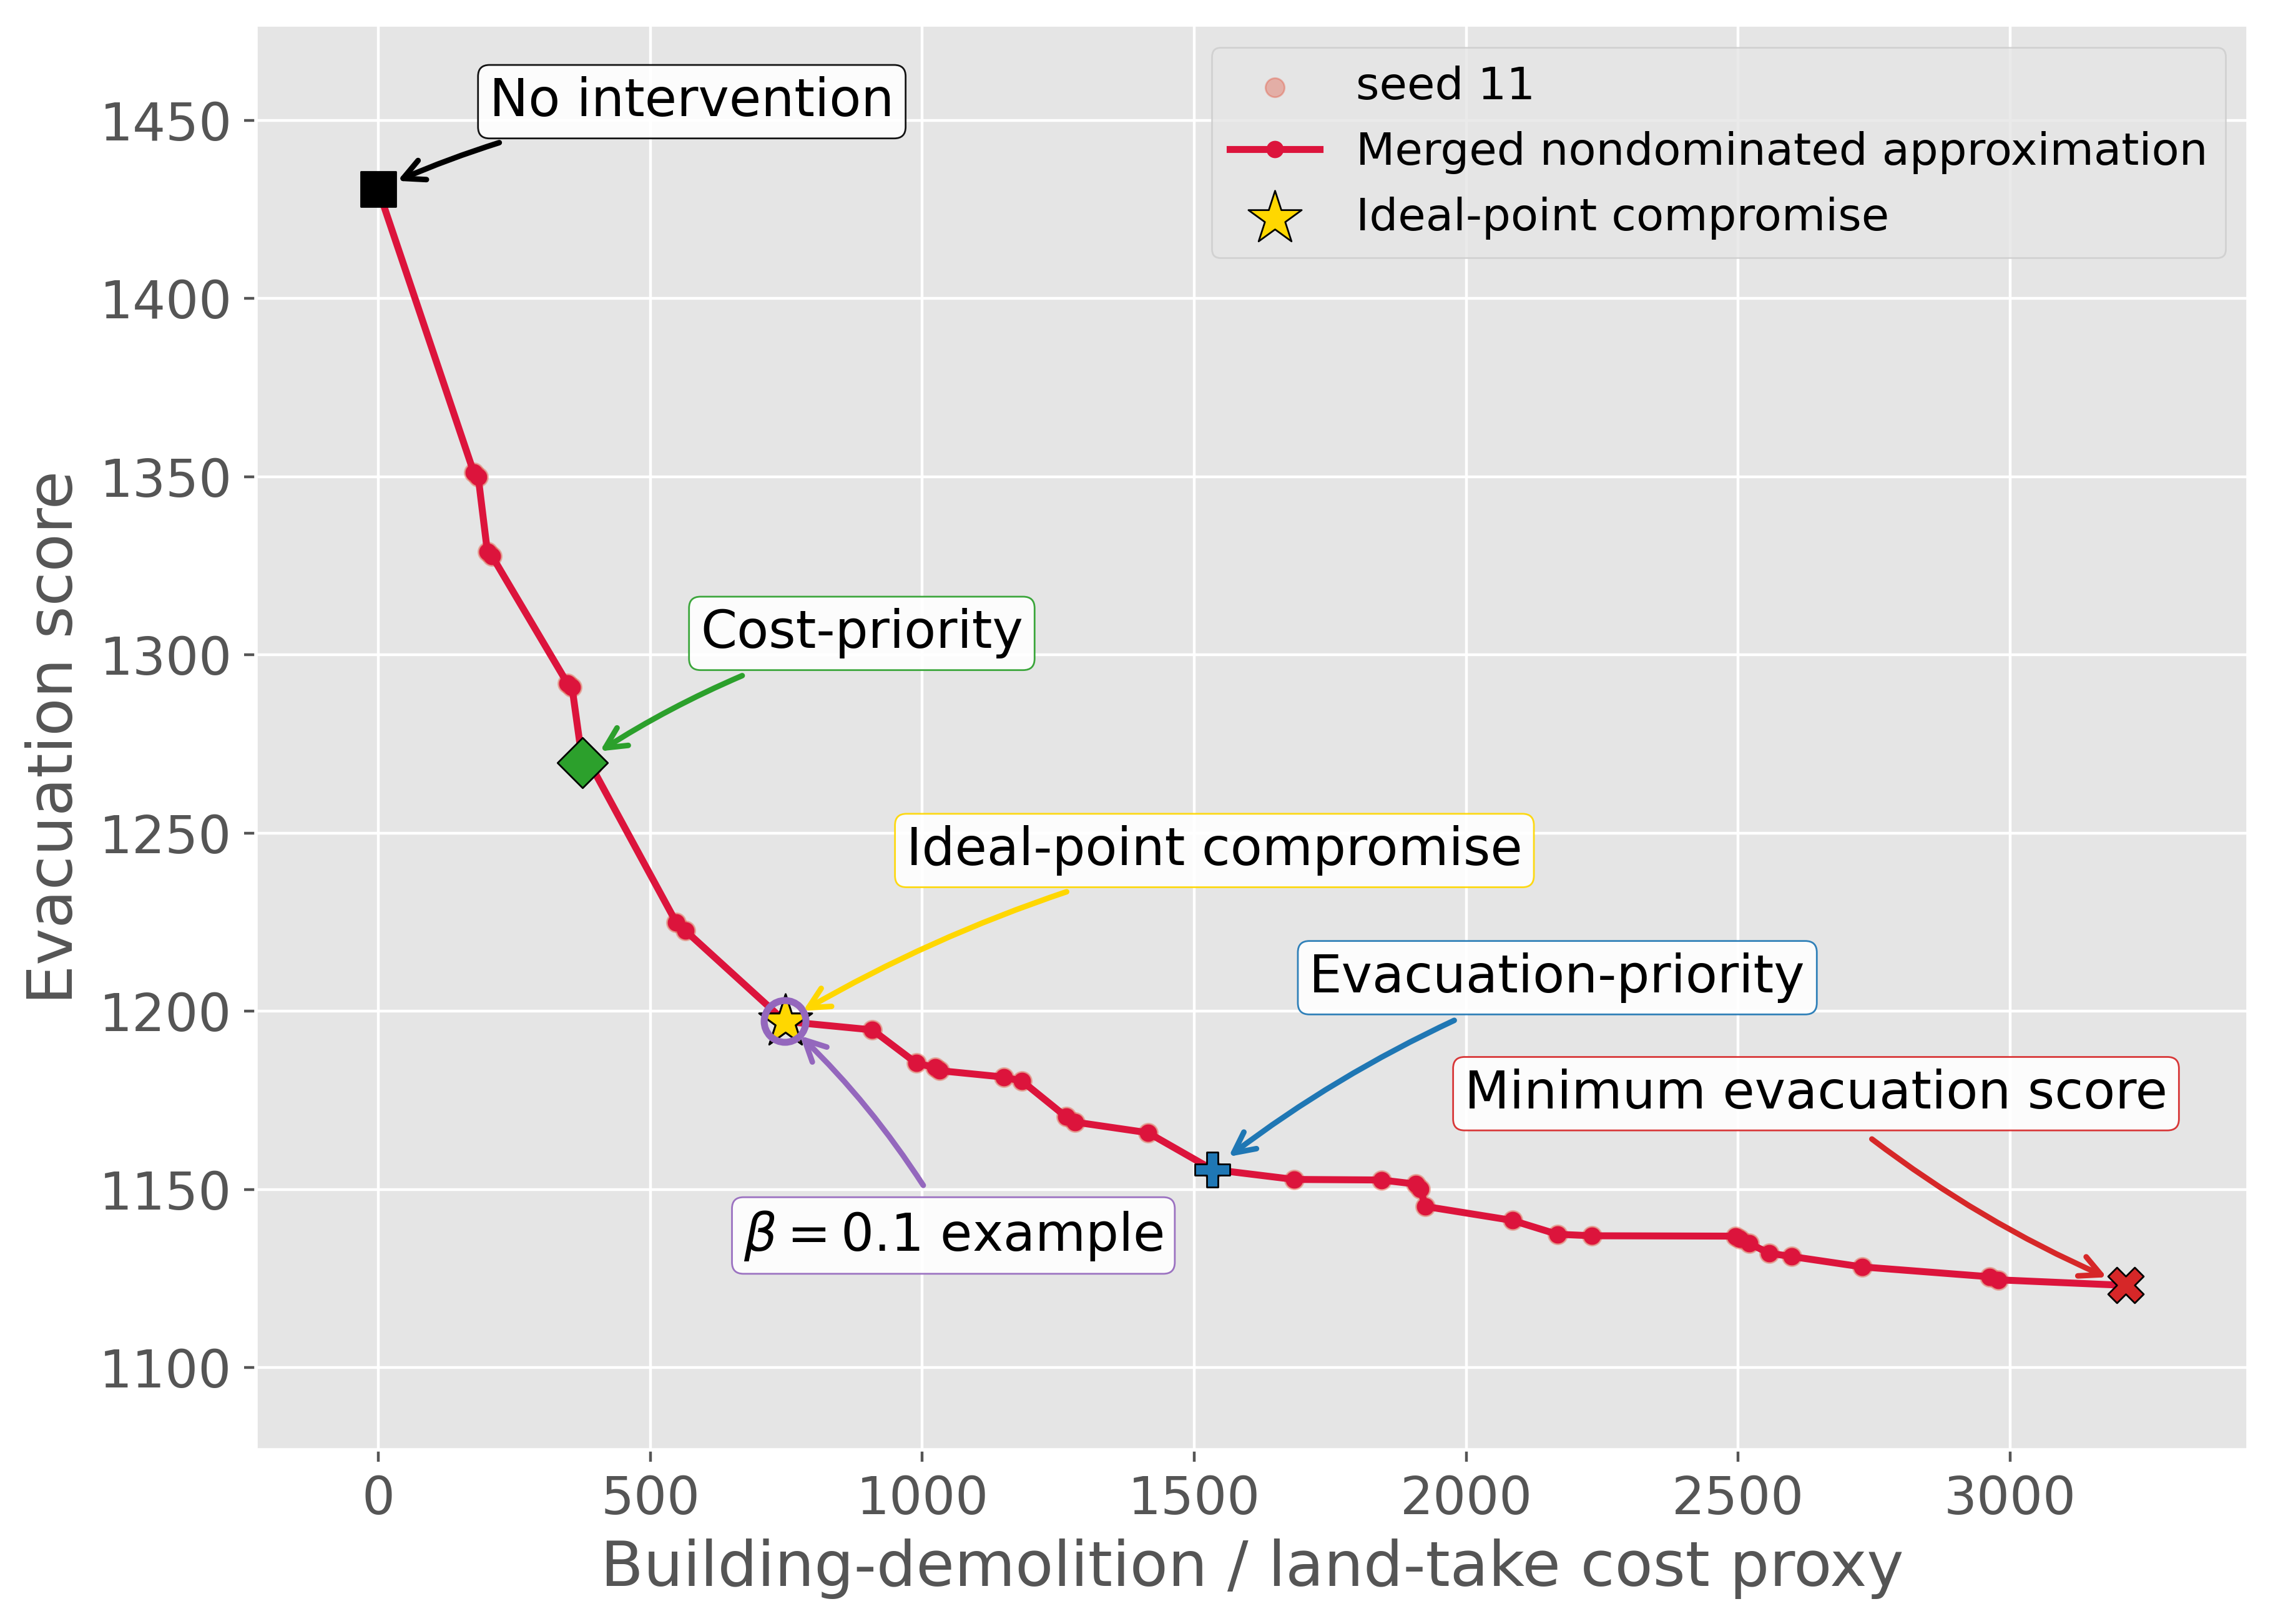
\includegraphics[width=0.70\linewidth]{fig/Fig_R2_pareto_front_15d.png}
\caption{Finite-budget NSGA-II Pareto-front approximation for the completed 15-segment seed-11 run. The full retained trade-off set and representative preferences are shown; unfinished seeds are not included or presented as completed evidence.}
\label{fig:pareto_15d}
\end{figure}


\begin{table}[htbp]
\centering
\caption{Experimental parameter settings.}
\label{tab:exp_params_revised}
\resizebox{\linewidth}{!}{%
\begin{tabular}{l c}
\hline
\textbf{Category} & \textbf{Value} \\
\hline
\multicolumn{2}{l}{\textit{Scenario and simulation}} \\
\hline
Project / scenario ID & \texttt{shipai\_0} (baseline) \\
Crowd size & 50{,}000 agents \\
Raster resolution & $0.1$ m \\
Simulator & C++ executable (\texttt{./260624}) \\
\hline
\multicolumn{2}{l}{\textit{Decision variables}} \\
\hline
Number of bottleneck segments & $K{=}15$ \\
Widening set & $\mathcal{D}=\{0,2,4\}$ m \\
\hline
\multicolumn{2}{l}{\textit{Objective function}} \\
\hline
Evacuation weight & $\alpha = 1.0$ \\
Illustrative post-hoc preference & $\beta = 0.1$ (not used to construct the front) \\
Reconstruction-cost coefficient & $c = 1.0$ (relative unit/m$^{2}$) \\
\hline
\multicolumn{2}{l}{\textit{Evolutionary algorithm}} \\
\hline
Population size & 40 \\
Offspring batches & 25 \\
Selection strategy & Rank--crowding binary tournament \\
Crossover operator (prob.) & Uniform crossover ($p_c=0.8$) \\
Mutation operator (prob.) & Gene-wise discrete replacement ($p_m=0.08$) \\
Environmental selection & $(\mu+\lambda)$ NSGA-II selection \\
Simulator calls per optimizer seed & $40+25\times40=1040$ \\
\revb{Completed main-run seed reported here} & \revb{11} \\
\revb{Completed main-run simulator calls} & \revb{1040} \\
\hline
\end{tabular}
}
\end{table}

{\color{blue}





\begin{table}[htbp]
\centering
\revfloat
\caption{Representative preferences on the completed 15-segment nondominated approximation.}
\label{tab:pareto_representatives}
\resizebox{\linewidth}{!}{%
\begin{tabular}{lccc}
\toprule
Preference & $F_{\mathrm{cost}}$ & $F_{\mathrm{evac}}$ & Selected segments (width) \\
\midrule
No intervention & 0.00 & 1430.61 & None \\
Reconstruction-cost priority & 375.19 & 1269.76 & R3 (2~m), R13 (2~m) \\
Ideal-point compromise & 747.52 & 1197.17 & R3 (4~m), R13 (4~m) \\
Evacuation-priority & 1532.90 & 1155.65 & R3 (4~m), R11 (2~m), R13 (4~m), R14 (4~m) \\
$\beta=0.1$ example & 747.52 & 1197.17 & R3 (4~m), R13 (4~m) \\
\bottomrule
\end{tabular}
}
\end{table}

The completed 15-segment seed-11 run retained 39 unique nondominated points after 1,040 real simulator calls (Figure~\ref{fig:pareto_15d}). The no-intervention case had an evacuation score of 1430.61 and zero reconstruction cost. The representative prioritizing reconstruction cost, $(F_{\mathrm{cost}},F_{\mathrm{evac}})=(375.19,1269.76)$, widens R3 and R13 by 2~m. The normalized ideal-point compromise $(747.52,1197.17)$ widens R3 and R13 by 4~m, while the evacuation-priority representative $(1532.90,1155.65)$ widens R3, R11, R13, and R14. Within the 39-point nondominated approximation retained by this completed seed-11 NSGA-II run, post-hoc minimization of $F_{\mathrm{evac}}+0.1F_{\mathrm{cost}}$ selects $(747.52,1197.17)$, which is also the point nearest the normalized ideal. This run-specific coincidence should not be interpreted as reproducing the different solution obtained by the legacy weighted-sum GA---R3 widened by 2~m and R13 by 4~m---or as identifying a unique global optimum.

The final Hypervolume for the completed run was $5.050\times10^6$, compared with $4.339\times10^6$ after the initial 40 evaluations. Because only seed 11 completed the full 50,000-agent budget at the time of this revision, Figure~\ref{fig:pareto_15d} is presented as a completed-seed approximation and no multi-seed main-front stability claim is made. The separate equal-budget parameter study in Section~\ref{sec:sensitivity_revised} uses three completed optimizer seeds.
}

{\color{blue}
\subsection{Village-scale Macro Verification and Plausibility Assessment}
\label{sec:macro_verification}

Following the baseline diagnosis in Section~\ref{sec:baseline} and the identification of representative Pareto solutions
in Section~\ref{sec:exp_setup}, we apply the case-scale verification protocol defined in
Section~\ref{sec:case_scale_protocol}. Direct observations of a full-community emergency evacuation and building-level
occupancy data are unavailable for Shipai Village. We therefore compare the baseline layout with the ideal-point
compromise intervention using five paired initial-position seeds (11, 29, 47, 71, and 101), 50,000 pedestrians per run,
and a stopping criterion of at least 95\% clearance. For each seed, the same initial-coordinate file is used for both
layouts. The representative intervention widens R3 and R13 by 4~m and is evaluated here as a diagnostic intervention;
the paired comparison does not constitute a multi-seed optimization campaign.

Table~\ref{tab:macro_validation} summarizes the paired temporal metrics. Across the five seeds, the reduction increases
from $t_{50}$ to $t_{95}$ and the normalized population-time also decreases, indicating that the intervention mainly
shortens the congestion-dominated tail.

\begin{table}[htbp]
\centering
\revfloat
\caption{Paired village-scale macro-verification results across five shared initial-position seeds.}
\label{tab:macro_validation}
\resizebox{\linewidth}{!}{%
\begin{tabular}{lccc}
\toprule
Metric & Baseline layout & Representative intervention & Paired reduction \\
\midrule
$t_{50}$ (s) & $414.82\pm2.18$ & $385.93\pm2.08$ & $6.96\%\pm0.13\%$ \\
$t_{80}$ (s) & $951.97\pm7.37$ & $792.07\pm8.06$ & $16.80\%\pm0.41\%$ \\
$t_{95}$ (s) & $1913.22\pm18.79$ & $1418.98\pm27.24$ & $25.84\%\pm0.82\%$ \\
Normalized population-time (s) & $580.33\pm4.10$ & $483.34\pm4.53$ & $16.71\%\pm0.21\%$ \\
\bottomrule
\end{tabular}
}
\end{table}





\begin{figure}[htbp]
\centering
\revfloat

\includegraphics[width=0.96\linewidth]{fig/FigR_C1_free_flow_lower_bound.png}
\caption{Actual-path free-flow plausibility assessment. Panels (a) and (b) show hexbin counts of simulated evacuation time against the actual-path lower bound for the original and intervention layouts; the red line denotes equality. Panel (c) compares probability-density distributions of $R_i=T_{\mathrm{actual},i}/T_{\mathrm{LB},i}$ pooled across five seeds. Panel (d) shows seed-specific distributions of $\Delta T_i=T_{\mathrm{actual},i}-T_{\mathrm{LB},i}$: B and O denote original and intervention layouts, the center line is the median, boxes span the interquartile range, whiskers extend to 1.5 interquartile ranges, and outliers are not displayed.}
\label{fig:free_flow_lower_bound}
\end{figure}

For each completed pedestrian $i$ with a positive actual path length, we calculate an actual-path free-flow lower bound,
\begin{equation}
T_{\mathrm{LB},i}=D_{\mathrm{actual},i}/1.6,
\label{eq:free_flow_lower_bound}
\end{equation}
where $D_{\mathrm{actual},i}$ is the simulated path length and 1.6~m/s is the maximum speed allowed by the simulator.
Because no pedestrian can traverse its realized path faster than this bound, $T_{\mathrm{actual},i}<T_{\mathrm{LB},i}$
would indicate a timing, distance, or speed-cap inconsistency. Panels~(a) and (b) compare the two quantities for all five
seeds; the red equality line marks the theoretical lower limit.

Panel~(c) reports the probability-density distribution of the dimensionless ratio
$R_i=T_{\mathrm{actual},i}/T_{\mathrm{LB},i}$ after pooling the qualifying pedestrians across the five seeds within each
layout. The area under each density is one, and a leftward shift indicates less time above the actual-path free-flow
benchmark. The mean of the five seed-level median ratios decreases from $4.745$ ($\mathrm{SD}=0.022$) in the original layout
to $4.529$ ($\mathrm{SD}=0.024$) under the representative intervention. This is a reduction in relative delay, not a 4.55\%
reduction in absolute evacuation time, because the denominator depends on each pedestrian's realized path length.

Panel~(d) instead measures the absolute delay above the same lower bound,
\begin{equation}
\Delta T_i=T_{\mathrm{actual},i}-T_{\mathrm{LB},i}.
\label{eq:free_flow_delay}
\end{equation}
Labels B11--B101 denote the five original-layout runs and O11--O101 the five corresponding intervention runs. In each
boxplot, the center line is the median, the box spans the first to third quartiles, and the whiskers extend to the most
extreme observations within 1.5 interquartile ranges; outliers are omitted from display. ``Paired seed'' means that each
B--O pair uses the same initial coordinates, not that the boxes show pedestrian-level paired differences. Across seeds,
the median delay decreases from $307.86\pm1.68$~s to $283.72\pm1.76$~s, while the 90th-percentile delay decreases from
$1055.40\pm13.41$~s to $787.93\pm10.78$~s. The stronger reduction in the upper tail is consistent with the larger reduction
in $t_{95}$ than in $t_{50}$. No qualifying pedestrian violates the lower bound under a 0.2~s numerical tolerance.
These diagnostics support internal macro-scale consistency, but they do not replace unavailable field validation. The
50,000-person total is supported by public demographic reports, whereas the within-village allocation remains a scenario
assumption.





\begin{figure}[htbp]
\centering
\revfloat

\includegraphics[width=1.0\linewidth]{fig/Fig_R1_macro_spatial_composite.png}
\caption{Complementary village-scale spatial and process assessment across five paired seeds: (a) original-layout and (b) representative-intervention median evacuation times by 5~m initial-position cell; (c) paired change (intervention minus original), where negative values indicate faster evacuation and the strongest reductions are concentrated in the central and central-eastern corridors; and (d) residual-population processes, with thick curves denoting across-seed medians and thin curves denoting individual runs.}
\label{fig:macro_spatial_composite}
\end{figure}



Having established the individual-level plausibility of the simulated times, Figure~\ref{fig:macro_spatial_composite}
provides a complementary village-scale view of where the intervention produces the aggregate improvement. Panels~(a)
and (b) compare 5~m-cell median evacuation times on a common scale, panel~(c) maps the paired change, and panel~(d)
shows the corresponding residual-population processes. The dominant negative changes in panel~(c) are concentrated in
the central and central-eastern corridors. Thus, the layout modification primarily reduces the high evacuation times
associated with the central congestion zone, rather than producing a spatially uniform reduction throughout the village.
A small number of positive cells indicate limited local redistribution of delay and do not alter this dominant spatial
pattern.
\FloatBarrier
}


{\color{blue}
\subsection{Sensitivity Analysis}
\label{sec:sensitivity_revised}

\subsubsection{Crowd-model and physical-parameter sensitivity}

We use a two-stage one-factor-at-a-time (OFAT) analysis to distinguish sensitivity of the evacuation model from robustness of the planning decision. First, the zero-widening case measures how a physical-parameter perturbation changes the evacuation result itself. Second, the same perturbed model is used to evaluate both a fixed road-widening plan and a newly optimized plan. This separation is important because a change in the absolute evacuation metric does not by itself imply that the intervention benefit or the preferred intervention strategy has become unstable.

The tested crowd-model parameters are the post-normalization local-effect coefficient $k$, neighborhood length $h$, and density threshold $\rho_{\max}$. Each parameter is varied individually by $-10\%$, $-5\%$, $+5\%$, and $+10\%$ from the baseline $(k,h,\rho_{\max})=(1.0,2.4~\mathrm{m},4.0)$, giving 13 scenarios including the shared baseline. The Shipai geometry, 8,000-agent crowd, exits, 15-segment decision space, and all other settings are fixed. Each scenario is repeated with seeds 11, 29, and 47. Every optimization run uses the same 12-member initial population and 24 real simulator calls (12 initial evaluations and one offspring generation). The fixed plan widens R3 and R13 by 4~m; the re-optimized plan is the normalized ideal-point compromise from the seed-specific Pareto front.

Let $M_{s,r}^{0}$ denote the zero-widening evacuation metric for scenario $s$ and seed $r$, where lower is better. Evacuation-result sensitivity is $100(M_{s,r}^{0}-M_{0,r}^{0})/M_{0,r}^{0}$ relative to the seed-matched baseline; retained improvement for plan $q$ is $100(M_{s,r}^{0}-M_{s,r}^{q})/M_{s,r}^{0}$ within the same scenario. Values are reported as mean $\pm$ SD across three seeds. Strategy stability is assessed from the selected segments, discrete widths, and Jaccard similarity to the corresponding baseline compromise. Each cell in Figure~\ref{fig:physical_optimization_sensitivity}(d) is the mean selected width across the three seed-specific compromises, combining selection consistency and widening magnitude rather than frequency alone.

Figure~\ref{fig:physical_evacuation_metric_sensitivity} shows the first-stage effect on the evacuation result. The baseline zero-widening metric is $517.55\pm1.04$. Across the tested range, this metric changes from $-8.92\%$ to $+11.13\%$ relative to the seed-matched baseline. The central normalized sensitivities estimated from the $\pm5\%$ perturbations are $-0.362$ for $k$, $+1.040$ for $h$, and $-0.809$ for $\rho_{\max}$; the corresponding $\pm10\%$ estimates are $-0.359$, $+0.933$, and $-0.889$. Thus, $h$ and $\rho_{\max}$ have the largest absolute effects and $k$ the smallest.

\begin{figure}[htbp]
\centering
\revfloat

\includegraphics[width=0.98\linewidth]{fig/FigR_C5_physical_evacuation_metric_sensitivity.pdf}
\caption{Sensitivity of the zero-widening evacuation result to the three crowd-model parameters under uniform relative OFAT perturbations. Points and error bars show the mean $\pm$ SD across seeds 11, 29, and 47. Positive changes indicate a higher, and therefore worse, evacuation metric.}
\label{fig:physical_evacuation_metric_sensitivity}
\end{figure}

Figure~\ref{fig:physical_optimization_sensitivity} reports the second-stage effect on optimization. Despite the changes in the absolute evacuation result, the fixed baseline plan remains beneficial in every physical-parameter scenario, with evacuation improvements of $3.85\%$--$7.78\%$. The scenario-specific re-optimized compromise also remains beneficial throughout, retaining improvements of $3.88\%$--$7.59\%$. The re-optimized compromise need not outperform the fixed plan because it balances reconstruction cost and evacuation performance under a small, equal evaluation budget rather than minimizing evacuation alone.

The intervention strategy is more stable in location than in exact width. R3 and R13 dominate across all perturbations, with only isolated secondary selections at R6 or R14. Relative to the seed-matched baseline compromise, segment-set Jaccard similarity is 0.667--1.000 and width-weighted similarity is 0.544--1.000. Physical-parameter uncertainty therefore changes the absolute result and exact widths, but not the positive intervention benefit or the central R3--R13 strategy.

\begin{figure}[htbp]
\centering
\revfloat

\includegraphics[width=0.99\linewidth]{fig/FigR_C5_physical_optimization_sensitivity.pdf}
\caption{Robustness of the road-widening optimization to physical-parameter perturbations. Panels (a)--(c) compare the evacuation improvement retained by the fixed baseline plan and the scenario-specific re-optimized compromise (mean $\pm$ SD across three seeds). Panel (d) shows the mean selected widening width for each candidate road segment across the three seed-specific compromises; these values combine selection consistency and widening magnitude and are not selection frequencies.}
\label{fig:physical_optimization_sensitivity}
\end{figure}
\FloatBarrier

\subsubsection{NSGA-II optimization-parameter sensitivity}

Optimizer-parameter sensitivity is evaluated separately from crowd-model sensitivity because these parameters change the search process, not the evacuation response of a fixed road design. Under a fixed simulation budget, we test whether the attained trade-off between reconstruction cost and evacuation performance remains stable and whether the same widening segments are selected.

The baseline matches Table~\ref{tab:exp_params_revised}: population size $P=40$, crossover probability $p_c=0.80$, and per-gene mutation probability $p_m=0.08$. An OFAT design tests $P\in\{20,40,60\}$, $p_c\in\{0.60,0.80,0.95\}$, and $p_m\in\{0.04,0.08,0.16\}$. The shared baseline gives seven unique configurations and 21 completed runs across seeds 11, 29, and 47. All runs use the main experiment's 15-segment decision space, widening set $\{0,2,4\}$~m, objectives, and simulator. For tractability, this controlled screen uses 15,000 agents and 240 real simulator calls per configuration and seed, rather than the 50,000 agents and 1,040 calls of the main run. After the initial population, $P=20$, 40, and 60 therefore receive 11, 5, and 3 offspring batches, respectively. Equalizing calls controls simulation cost, not the number of generations.

\begin{figure}[htbp]
\centering
\revfloat

\includegraphics[width=0.98\linewidth]{fig/FigR_C5_nsga2_parameter_sensitivity.pdf}
\caption{Equal-call NSGA-II parameter sensitivity across seeds 11, 29, and 47: (a) population size; (b) crossover probability; and (c) per-gene mutation probability. Points and error bars show mean $\pm$ SD of final Hypervolume computed with the common reference point $(F_{\mathrm{evac}},F_{\mathrm{cost}})=(2000,6000)$; higher values indicate a better attained objective-space trade-off.}
\label{fig:nsga2_parameter_sensitivity}
\end{figure}

Final fixed-reference Hypervolume measures the objective-space area dominated by the final nondominated approximation relative to $(F_{\mathrm{evac}},F_{\mathrm{cost}})=(2000,6000)$; higher is better. We report mean $\pm$ SD across seeds. Decision stability uses the normalized ideal-point compromise from each seed and the mean of its three pairwise segment-set Jaccard similarities, $|A\cap B|/|A\cup B|$, where 1 denotes identical selections and 0 denotes no overlap.

Figure~\ref{fig:nsga2_parameter_sensitivity} shows mean final Hypervolume from $8.802\times10^6$ ($P=60$) to $8.842\times10^6$ ($P=20$), with $8.835\times10^6$ at the baseline. The 0.45\% total spread indicates stable objective-space performance under the equal-call budget; it does not show that larger populations are intrinsically worse, because they receive fewer offspring batches. Mean Jaccard similarity ranges from 0.278 ($P=60$) to 0.639 ($P=20$), with 0.478 at the baseline. Thus, similar objective trade-offs can arise from different segment combinations. The experiment supports finite-budget objective-space robustness, but not a unique widening strategy, global convergence, or parameter independence.


\FloatBarrier
}

{\color{blue}
\subsection{Computational Performance}
\label{sec:computational_performance}

All experiments were conducted on a workstation with an Intel Core Ultra 9 285K CPU (20 cores), an NVIDIA GeForce RTX
5090 GPU with 32~GB memory, and CUDA 13.0. The corrected \texttt{260624} CUDA/C++ simulator uses a uniform spatial hash
for local neighbor queries, while a Python driver coordinates the optimization. Runtime tests used the fixed Shipai domain
with the same initialization, exits, and stopping criterion, with two timed repetitions for each population.

\begin{table}[htbp]
\centering
\revfloat
\caption{Empirical end-to-end runtime in the fixed Shipai domain using the corrected \texttt{260624} simulator (two timed repetitions per population).}
\label{tab:runtime_scaling}
\begin{tabular}{rcc}
\toprule
Agents & Mean wall time (s) & SD (s) \\
\midrule
5,000 & 6.55 & 0.04 \\
10,000 & 7.49 & 0.08 \\
20,000 & 9.89 & 0.21 \\
50,000 & 22.12 & 0.39 \\
100,000 & 51.33 & 0.36 \\
\bottomrule
\end{tabular}
\end{table}

As shown in Table~\ref{tab:runtime_scaling}, the mean runtime was 22.12~s for 50,000 agents and 51.33~s for 100,000 agents.
These results demonstrate that the corrected GPU simulator can efficiently support large community-scale evacuation
simulations.

The completed 15-segment, seed-11 NSGA-II run used a population of 40 over 25 offspring batches. It required 1,040 real
50,000-agent simulations and took 21,824.565~s (approximately 6.06~h), averaging 20.99~s per evaluation including
optimization overhead. This efficiency supports the use of the framework as an offline planning and road-network
optimization tool.
\FloatBarrier
}

{\color{blue}
\section{Discussion}
\label{sec:discussion_revised}

\subsection{Scope, transferability, and geographic scalability}

The primary application domain is high-density urban villages in southern China, where narrow alleys, irregular road networks, and limited emergency access create a continuing need for targeted micro-regeneration. Although this study evaluates emergency evacuation, widening critical passages may also support daily pedestrian circulation and emergency access; these possible co-benefits were not measured here.

The simulation--diagnosis--optimization workflow can be transferred to other constrained spatial systems only after redefining interventions and recalibrating inputs. In wildland--urban interface communities, relevant decisions would include road-network redundancy, alternative egress, intersection capacity, topological connectivity, safe areas, vehicle evacuation, and time-varying wildfire conditions. In large indoor complexes, variables would concern corridors, doors, stairs, and exits, with additional calibration for vertical circulation, indoor regulations, and occupant behavior. These settings share computational representations of constrained movement and bottlenecks, but neither has been validated in the present study.

The population-scaling results in Section~\ref{sec:computational_performance} increase agent count within a fixed Shipai domain. They do not validate expansion to a larger geographic area. Larger domains would additionally require spatial partitioning, adaptive or multi-resolution grids, hierarchical routing, distributed candidate evaluation, and renewed validation of population allocation and route choice.

\subsection{Limitations and future multi-hazard extensions}

Dynamic fire, flood, or earthquake coupling remains future work. Although a fire-propagation cellular-automaton interface exists in the broader code base, the present experiments do not connect a time-varying hazard field to pedestrian accessibility, perception, potential fields, or rerouting. A defensible multi-hazard extension requires interacting layers for hazard propagation, exposure and perception, behavioral response, dynamic path choice, and possibly two-way feedback. Each layer would require independent calibration and validation before operational use.

The validation is also limited by the absence of full-community evacuation observations and building-level occupancy data. The macro assessment therefore provides paired multi-seed consistency, spatial response, and lower-bound plausibility evidence, not direct validation of the absolute clearance time. Physical-parameter sensitivity shows that absolute outputs and exact intervention choices retain uncertainty. Finally, the completed 50,000-agent main Pareto result currently represents one full optimizer seed; multi-seed front stability should be updated when the remaining equal-budget main runs are complete.
}


\section{Conclusion}
\label{sec:conclusion}

This work presents a simulation-driven, targeted micro-regeneration framework for improving evacuation performance in
high-density urban informal settlements with narrow and irregular road networks. We first build a high-resolution raster environment
from GIS layers and perform a baseline SPH-based evacuation simulation to reveal persistent congestion hotspots. Based on
cumulative congestion time and cumulative congestion density, we identify critical bottlenecks and map them to candidate
road segments for intervention. We then formulate a discrete widening optimization problem with realistic construction
templates and solve it using a simulation-in-the-loop \revb{multi-objective NSGA-II}, explicitly balancing evacuation benefit and
demolition/land-take proxy.

A key contribution is the hierarchical calibration and validation of the SPH-based movement model. By fitting empirical
fundamental-diagram data and validating corridor-level speed--density--flow relationships, we provide micro-level evidence
that the simulator reproduces essential pedestrian movement paradigms in constrained spaces. \revb{At the village scale,
paired multi-seed simulations and free-flow plausibility checks provide scenario-based consistency evidence rather than direct
validation of absolute clearance times.} In the Shipai Village case study, the optimized widening scheme yields a clear
reduction in evacuation time and congestion severity while requiring only localized interventions, highlighting strong
spatial heterogeneity in marginal widening benefits. \revb{The finite-budget Pareto front provides an alternative prioritizing reconstruction cost, an ideal-point compromise, and an evacuation-priority alternative, while the sensitivity analyses show that objective-space performance is comparatively
robust but the exact road selection retains uncertainty.}

The proposed framework is practical for planning scenarios where large-scale field evacuation validation is infeasible. It
provides not only quantitative performance improvements but also interpretable spatial guidance on where limited budgets
should be allocated. \revb{The measured computational cost positions the framework as an offline planning tool rather than a
real-time control system.} Future work will extend the method to multi-scenario and multi-hazard settings (e.g., varying exit
availability, population distributions, and hazard evolution), incorporate richer behavioral heterogeneity and compliance,
and \revb{strengthen multi-seed Pareto analysis, computational scaling, and dynamically coupled multi-hazard validation.}

\section*{Declaration of generative AI and AI-assisted technologies in the writing process} 
During the preparation of this work the authors used ChatGPT for language polishing. After using this tool, the authors reviewed and edited the content as needed and take full responsibility for the content of the publication.

\ifanonymous
\else
\section*{Acknowledgments}
This work was supported by the Guangdong Provincial Project (No. 2023QN10H717),
the Guangzhou--HKUST(GZ) Joint Funding Program (No. 2025A03J3639),
and the AI Research and Learning Base of Urban Culture Project (No. 2023WZJD008).
\fi

\bibliographystyle{elsarticle-harv} % 或 unsrt
% \bibliographystyle{splncs04}   % Springer LNCS 专用样式
\bibliography{reference}      % 只写文件名，不写 .bib
\end{document}
